\documentclass[a4paper,10pt]{extarticle}
\usepackage[ngerman]{babel}
\usepackage{amsmath,amsthm}
\usepackage{ascii}
\usepackage[adobe-utopia]{mathdesign}
\usepackage[T1]{fontenc}
\usepackage[margin=0.5cm]{geometry}
\usepackage{multicol}
\usepackage{color,graphicx,overpic}
\usepackage{hyperref}
%Enumerator
\usepackage[inline]{enumitem}
%Table imports
\newcommand{\ra}[1]{\renewcommand{\arraystretch}{#1}}
%Style imports
\usepackage{enumitem}
\usepackage{tcolorbox}
\usepackage{listings}
\usepackage{minted}
\usepackage{algorithm}
\usepackage{algpseudocode}
\usepackage{authblk}
\usepackage{fancyhdr}
\usepackage{fancyhdr}
\usepackage{datetime}
\usepackage[iso,german]{isodate}
%Graphic imports
\usepackage{tikz}
\graphicspath{ {./img/} }
% Turn off header and footer
\pagestyle{empty}

% Redefine section commands to use less space
\makeatletter
\renewcommand{\section}{\@startsection{section}{1}{0mm}%
                                {-1ex plus -.5ex minus -.2ex}%
                                {0.5ex plus .2ex}%x
                                {\normalfont\large\bfseries}}
\renewcommand{\subsection}{\@startsection{subsection}{2}{0mm}%
                                {-1explus -.5ex minus -.2ex}%
                                {0.5ex plus .2ex}%
                                {\normalfont\normalsize\bfseries}}
\renewcommand{\subsubsection}{\@startsection{subsubsection}{3}{0mm}%
                                {-1ex plus -.5ex minus -.2ex}%
                                {1ex plus .2ex}%
                                {\normalfont\small\bfseries}}
\renewcommand{\paragraph}{%
  \@startsection{paragraph}{4}%
  {\z@}{1ex \@plus 1ex \@minus .2ex}{-1em}%
  {\normalfont\normalsize\bfseries}%
}
\makeatother

% Define BibTeX command
\def\BibTeX{{\rm B\kern-.05em{\sc i\kern-.025em b}\kern-.08em
    T\kern-.1667em\lower.7ex\hbox{E}\kern-.125emX}}

% Don't print section numbers
\setcounter{secnumdepth}{0}

\setlength{\parindent}{0pt}
\setlength{\parskip}{0pt plus 0.5ex}

%My Environments
\newtheorem{example}[section]{Example}
% -----------------------------------------------------------------------
\definecolor{codegreen}{rgb}{0,0.6,0}
\definecolor{codegray}{rgb}{0.5,0.5,0.5}
\definecolor{codepurple}{rgb}{0.58,0,0.82}
\definecolor{backcolour}{rgb}{0.95,0.95,0.92}
\lstdefinelanguage{CSS}{
  morekeywords={accelerator,azimuth,background,background-attachment,
    background-color,background-image,background-position,
    background-position-x,background-position-y,background-repeat,
    behavior,border,border-bottom,border-bottom-color,
    border-bottom-style,border-bottom-width,border-collapse,
    border-color,border-left,border-left-color,border-left-style,
    border-left-width,border-right,border-right-color,
    border-right-style,border-right-width,border-spacing,
    border-style,border-top,border-top-color,border-top-style,
    border-top-width,border-width,bottom,caption-side,clear,
    clip,color,content,counter-increment,counter-reset,cue,
    cue-after,cue-before,cursor,direction,display,elevation,
    empty-cells,filter,float,font,font-family,font-size,
    font-size-adjust,font-stretch,font-style,font-variant,
    font-weight,height,ime-mode,include-source,
    layer-background-color,layer-background-image,layout-flow,
    layout-grid,layout-grid-char,layout-grid-char-spacing,
    layout-grid-line,layout-grid-mode,layout-grid-type,left,
    letter-spacing,line-break,line-height,list-style,
    list-style-image,list-style-position,list-style-type,margin,
    margin-bottom,margin-left,margin-right,margin-top,
    marker-offset,marks,max-height,max-width,min-height,
    min-width,-moz-binding,-moz-border-radius,
    -moz-border-radius-topleft,-moz-border-radius-topright,
    -moz-border-radius-bottomright,-moz-border-radius-bottomleft,
    -moz-border-top-colors,-moz-border-right-colors,
    -moz-border-bottom-colors,-moz-border-left-colors,-moz-opacity,
    -moz-outline,-moz-outline-color,-moz-outline-style,
    -moz-outline-width,-moz-user-focus,-moz-user-input,
    -moz-user-modify,-moz-user-select,orphans,outline,
    outline-color,outline-style,outline-width,overflow,
    overflow-X,overflow-Y,padding,padding-bottom,padding-left,
    padding-right,padding-top,page,page-break-after,
    page-break-before,page-break-inside,pause,pause-after,
    pause-before,pitch,pitch-range,play-during,position,quotes,
    -replace,richness,right,ruby-align,ruby-overhang,
    ruby-position,-set-link-source,size,speak,speak-header,
    speak-numeral,speak-punctuation,speech-rate,stress,
    scrollbar-arrow-color,scrollbar-base-color,
    scrollbar-dark-shadow-color,scrollbar-face-color,
    scrollbar-highlight-color,scrollbar-shadow-color,
    scrollbar-3d-light-color,scrollbar-track-color,table-layout,
    text-align,text-align-last,text-decoration,text-indent,
    text-justify,text-overflow,text-shadow,text-transform,
    text-autospace,text-kashida-space,text-underline-position,top,
    unicode-bidi,-use-link-source,vertical-align,visibility,
    voice-family,volume,white-space,widows,width,word-break,
    word-spacing,word-wrap,writing-mode,z-index,zoom},
  morestring=[s]{:}{;},
  sensitive,
  morecomment=[s]{/*}{*/}
}
%=====================================SCSS=========================================
\lstdefinelanguage{SCSS}{
    morekeywords={accelerator,azimuth,background,background-attachment,
    background-color,background-image,background-position,
    background-position-x,background-position-y,background-repeat,
    behavior,border,border-bottom,border-bottom-color,
    border-bottom-style,border-bottom-width,border-collapse,
    border-color,border-left,border-left-color,border-left-style,
    border-left-width,border-right,border-right-color,
    border-right-style,border-right-width,border-spacing,
    border-style,border-top,border-top-color,border-top-style,
    border-top-width,border-width,bottom,caption-side,clear,
    clip,color,content,counter-increment,counter-reset,cue,
    cue-after,cue-before,cursor,direction,display,elevation,
    empty-cells,filter,float,font,font-family,font-size,
    font-size-adjust,font-stretch,font-style,font-variant,
    font-weight,height,ime-mode,include-source,
    layer-background-color,layer-background-image,layout-flow,
    layout-grid,layout-grid-char,layout-grid-char-spacing,
    layout-grid-line,layout-grid-mode,layout-grid-type,left,
    letter-spacing,line-break,line-height,list-style,
    list-style-image,list-style-position,list-style-type,margin,
    margin-bottom,margin-left,margin-right,margin-top,
    marker-offset,marks,max-height,max-width,min-height,
    min-width,-moz-binding,-moz-border-radius,
    -moz-border-radius-topleft,-moz-border-radius-topright,
    -moz-border-radius-bottomright,-moz-border-radius-bottomleft,
    -moz-border-top-colors,-moz-border-right-colors,
    -moz-border-bottom-colors,-moz-border-left-colors,-moz-opacity,
    -moz-outline,-moz-outline-color,-moz-outline-style,
    -moz-outline-width,-moz-user-focus,-moz-user-input,
    -moz-user-modify,-moz-user-select,orphans,outline,
    outline-color,outline-style,outline-width,overflow,
    overflow-X,overflow-Y,padding,padding-bottom,padding-left,
    padding-right,padding-top,page,page-break-after,
    page-break-before,page-break-inside,pause,pause-after,
    pause-before,pitch,pitch-range,play-during,position,quotes,
    -replace,richness,right,ruby-align,ruby-overhang,
    ruby-position,-set-link-source,size,speak,speak-header,
    speak-numeral,speak-punctuation,speech-rate,stress,
    scrollbar-arrow-color,scrollbar-base-color,
    scrollbar-dark-shadow-color,scrollbar-face-color,
    scrollbar-highlight-color,scrollbar-shadow-color,
    scrollbar-3d-light-color,scrollbar-track-color,table-layout,
    text-align,text-align-last,text-decoration,text-indent,
    text-justify,text-overflow,text-shadow,text-transform,
    text-autospace,text-kashida-space,text-underline-position,top,
    unicode-bidi,-use-link-source,vertical-align,visibility,
    voice-family,volume,white-space,widows,width,word-break,
    word-spacing,word-wrap,writing-mode,z-index,zoom},
    comment=[l]{//},
    ndkeywords = {@mixin}
}
%==================================Javascript======================================
\lstdefinelanguage{JavaScript}{
  keywords={typeof, new, true, false, catch, function, return, null, catch, switch, var, if, in, while, do, else, case, break},
  ndkeywords={class, export, boolean, throw, implements, import, this},
  sensitive=false,
  comment=[l]{//},
  morecomment=[s]{/*}{*/},
  morestring=[b]',
  morestring=[b]"
}
\lstdefinestyle{sharpc}{language=[Sharp]C}
\lstset{ %
    backgroundcolor=\color{backcolour},   
    commentstyle=\color{codegreen},
    keywordstyle=\color{magenta},
    numberstyle=\tiny\color{codegray},
    stringstyle=\color{codepurple},
    basicstyle=\scriptsize,
    breakatwhitespace=false,         
    breaklines=true,                 
    captionpos=b,                    
    keepspaces=true,                 
    numbers=none,                    
    numbersep=5pt,                  
    showspaces=false,                
    showstringspaces=false,
    showtabs=false,                  
    tabsize=2,
    frame=single,
    language=[Sharp]C,
    postbreak=\raisebox{0ex}[0ex][0ex]{\ensuremath{\color{black}\hookrightarrow\space}}
}
\algrenewcommand\algorithmicfunction{\textbf{algorithm}}
\newcommand{\code}[1]{\texttt{#1}}
\title{Mobile and GUI Engineering\\\Large WPF}
\author{Oliviero Chiodo\\ Stefano Kals}
\date{Herbstsemester 2015}
\affil{Hochschule für Technik Rapperswil}
\begin{document}
\raggedright
\footnotesize
\begin{multicols*}{3}

% multicol parameters
% These lengths are set only within the two main columns
%\setlength{\columnseprule}{0.25pt}
\setlength{\premulticols}{1pt}
\setlength{\postmulticols}{1pt}
\setlength{\multicolsep}{1pt}
\setlength{\columnsep}{2pt}
\section{Grundlagen der GUI Programmierung}
Apps bestehen aus lose gekoppelten, wiederverwendbaren Komponenten. Diese sind Activities (für den Benutzer sichtbar) und Services, Content Provider, Broadcast Receivers (unsichtbar für Benutzer). Das System hat die Kontrolle über alle Applikationen und Verwaltet den Lebenszyklus, ist verantwortlich für die Kommunikation zwischen Komponenten und schliesst die Apps automatisch um Speicher zu sparen.
\paragraph{Activites} Dies sind die Hauptbausteine in der App Entwicklung, die Activity interagiert mit dem Benutzer. Eine Activity stellt immer auch einen möglichen Eintrittspunkt in die App ein.
\begin{lstlisting}[language=java]
public class MainActivity extends Activity {
  @Override
  protected void onCreate(Bundle savedInstanceState) {
    super.onCreate(savedInstanceState);
    /* ... */
  }
}
\end{lstlisting}
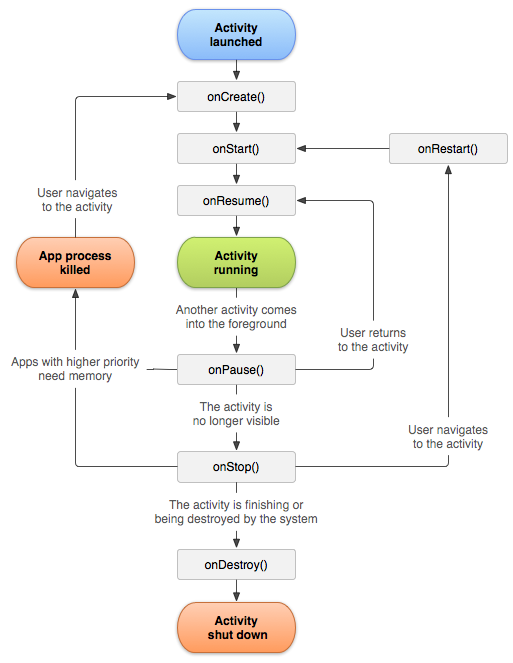
\includegraphics[scale=0.35]{activity_lifecycle.png}
Unterschied Paused/Resume: wird die Activity von einer anderen überdeckt (z.B. Notificationleiste heruntergezogen), wird die erste pausiert (\code{onPause}). Kommt sie wieder in den Vordergrund, wird wieder \code{onResume} aufgerufen.

\code{onPause} ist \textbf{garantiert}. \code{onStop} ist jedoch \textbf{nicht garantiert}. Darum:

\paragraph{Best Practice}

\begin{itemize}
  \item \code{onCreate} erstellt GUI beim Start.
  \item \code{onResume} reagiert auf Benutzereingaben.
  \item \code{onPause} sichert Daten (da die App auch im \code{onStop} oder \code{onDestroy} gekillt werden kann).
  \item \code{onStop} gibt Ressourcen frei.
\end{itemize}

Bei Konfigurationsänderungen wird die Activity neu gestartet. Dazu zählen z.B. \textbf{Screenausrichtungsänderungen}.

Stopped/Started: kommt die Activity wieder in den Vordergrund, weil der User die Applikation nochmal startet oder mit dem Back-Button zurückkommt, wird onRestart aufgerufen.

Destroyed: die App wird vom System destroyed, oder wenn sie explizit vom User geschlossen wird.

\paragraph{Stack}

Activities werden in einem Stack verwaltet, wobei die Activites eines Stacks zu verschiedenen Apps gehören können.\\ 
Eine Gruppe von Activities in einem Stack nennt man auch \textbf{Task}. Es können mehrere Tasks gleichzeitig existieren. Tasks lassen sich im Overview Screen anzeigen.

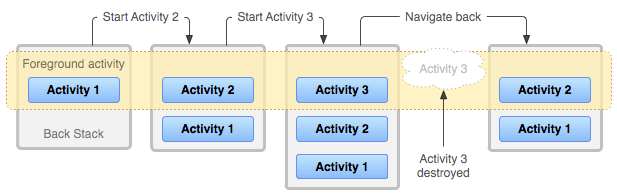
\includegraphics[scale=0.29]{diagram_backstack.png}

\paragraph{Activity Launch Modes} Activities haben verschiedene Launch Modes

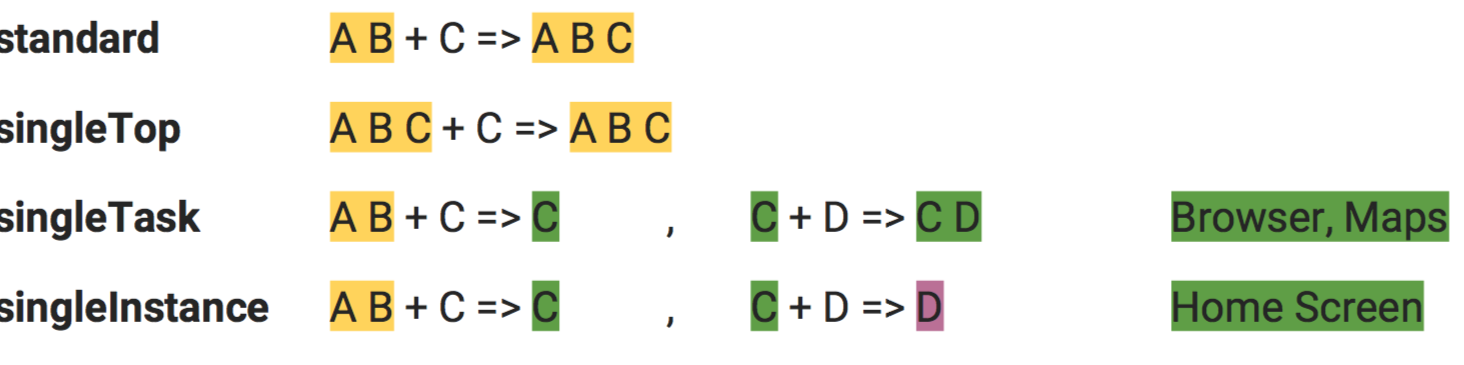
\includegraphics[scale=0.11]{activity-launch-modes.png}

\begin{itemize}
\item \textbf{Standard:} Es wird eine neue Activity in den Stack gepusht
\item \textbf{SingleTop:} Ist Activity A zuoberst auf dem Stack und sie wird nochmals gestartet, wird in Activity A \code{onNewIntent()} ausgeführt
\item \textbf{SingleTask:} Das System erstellt einen neuen Task und instanziert die Activity als die Root des neuen Tasks. Wenn aber schon eine Instanz dieser Activity existiert, wird \code{onNewIntent()} in dieser aufgerufen. 
\item \textbf{SingleInstance:} Es darf nur eine Instanz der Activity geben
\end{itemize}

\paragraph{APK}

Activities (und Ressourcen, etc) werden in ein APK gepackt und installiert. Wird eine Activity aktiv, wird pro APK ein Linux Prozess mit einem Thread gestartet, welcher alle Activities die indiesem APK enthalten sind ausführt. Jedes APK wird unter einem eigenen Linux-User installiert. Inhalt: Libraries, Ressourcen, Assets, Metadaten, kompilierte Klassen im DEX-Format.

Ein APK ist nichts anderes als ein JAR, welches wiederum eine ZIP-Datei ist.

\subsection{Application}
Parent unserer Activities im Manifest ist die Application. Ist auch eine Klasse, die den globalen Zustand unserer App hält. Kann durch eigene Application-Subklasser ersetzt werden. Zugriff aus Activity mit \code{getApplication}, Lifecycle-Methoden: \code{onCreate}, \code{onLowMemory}, \code{onConfigurationChanged}.


\paragraph{Intent} Ein Intent beschreibt was gemacht werden soll und das System entscheidet wer zuständig ist. Apps können selbst wiederum Activites zur Verfügung stellen und bestehende Applikationen ersetzen. Andere Activities können explizit oder implizit aufgerufen werden:
\begin{lstlisting}[language=java]
// Explizit mit Klasse
Intent in = new Intent(this, CalculateActivity.class)
// Implizit mit Aktion
Intent in = new Intent(MediaStore.ACTION_IMAGE_CAPUTRE)
\end{lstlisting}
Andere Activities kann man mit \code{startActivity(intent)} oder \code{startActivityForResult(intent, myId)} starten. Um bei letzterem mit dem Rückgabewert arbeiten zu können muss man \code{onActivityResult} überschreiben.
\begin{lstlisting}[language=java]
@Override
protected void onActivityResult(int request, int result, Intent data) {
  if (result == Activity.RESULT_OK && request == myId) {
    /* ... */
  }
}
\end{lstlisting}
Möchte man einem Intent Daten übergeben, kann man das entweder mit der \code{setData} Methode, welche eine URI entgegennimmt, oder mit \code{putExtra(MediaStore.EXTRA\_OUTPUT, imageCaptureUri)}. Letzere ist eine Struktur mit Key-Value Paaren und nimmt nur primitive Daten, Strings und serialisierbare Datentypen an.

\paragraph{Manifest} Das Manifest enthält Meta-Daten einer App. Es umfasst
\begin{itemize}
\item Komponenten der App
\item Metadaten (Name, Icon, Versionsnummer)
\item Permissions (Internet, kostenpflichtige Anrufe etc.)
\item Anforderungen an die Geräte API
\item \code{minSdkVersion} min-Version des Gerätes
\item \code{targetSdkVersion} höchste Version, mit der getestet wurde
\item Name der Singleton Instanz der Application (Sub-)Klasse.
\end{itemize}

Das Manifest wird vom System verwendet um zu wissen, ob die App installiert werden kann, welche Permissions diese verwendet etc.

\subsection{Android GUI}
\paragraph{Aufbau} Die Basisklasse um User Interfaces zu bauen ist die \code{View}. Eine View ist zuständig seinen Inhalt zu zeichnen und Events zu behandeln. Untergruppen der View sind Widgets und ViewGroups. Widgets ist ein Sammelbegriff für alle fix-fertigen Komponenten für User-Interfaces (Buttons, Images, Checkboxes etc.)
\paragraph{ViewGroup} Die ViewGroup ist eine Unterklasse von View. Sie kann andere View beinhalten. Wenn die ViewGroup beinhaltende View anordnet, spricht man von einem Layout.
\paragraph{Basis Layout} Layouts sind ViewGroups und beschreiben die visuelle Struktur des UIs.
\includegraphics[scale=0.45]{layouts.png}
Die Layout-Parameter beschreiben wie die Views angeordnet und dargestellt werden. Für alle ViewGroups gemeinsam sind \code{android:layout\_width} und \code{android:layout\_height}. Häufig benutze Werte sind \code{match\_parent} (So gross wie mögich, also wie der Parent erlaubt) und \code{wrap\_content} (so klein wie möglich, also wie die Kinder erlauben).\\
In einem \textbf{Linear Layout} werden die Elemente horizontal oder vertikal angeordnet. Mit \code{android:layout\_weight} kann man Elementen ein Gewicht geben, da es selten sinnvoll ist, alle Elemente gleich gross zu lassen. Kinder ohne Weight bekommen minimalen Platz, auf die restlichen wird der verfügbare Platz nach Gewicht aufgeteilt.\\
Das \textbf{Relative Layout} ist das vielseitigse Layout welches Kinder relative zueinander anordnet.
\begin{lstlisting}[language=xml]
<RelativeLayout xmlns:android="... >
  <TextView
    android:text="1. Platz"
    android:id=@+id/first"
    android:layout_centerHorizontal="true" />
  <TextView
    android:text="2. Platz"
    android:id="@+id/first"
    android:layout_below="@id/first"
    android:layout_toStartOf="@id/first" />
  <TextView
    android:text="3. Platz"
    android:id="@+id/textView3"
    android:layout_below="@id/first"
    android:layout_toEnfOf="@id/first" />
</RelativeLayout>
\end{lstlisting}
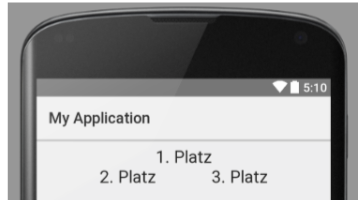
\includegraphics[scale=0.25]{RelativLayout.png} \\
Das \textbf{Frame Layout} kann die Kinder übereinander anordnen (Hilfslinien bei einer Kamera-App).\\
Das Layout muss in der Activity deklariert werden. Dies wird in der Activit Klasse mit \code{setContentView(R.layout.activity\_main)} gemacht.\\

\paragraph{Weitere Layouts}
\begin{itemize}
  \item FlexboxLayout: CSS Flexbox
  \item ConstraintLayout, mit RelativeLayout verwandt (war in Android Studio immer Standard ab irgendeiner Version)
  \item WebView um HTML anzuzeigen: JavaScript kann aktiviert werden, und Java-Objekte können mit JS angesprochen werden
\end{itemize}

\subsection{View finden}
\begin{lstlisting}[language=java]
Button button = (Button) findViewById(R.id.button)
\end{lstlisting}
findViewById innerhalb einer Activity sucht im aktuellen Layout (wahrscheinlich dasjenige von \code{setContentView}). Rückgabe ist immer die Oberklasse \code{View},  das Resultat muss also noch gecastet werden.

Hat man allerdings ein Fragment oder z.B. ein Listenelement, so muss man die Parent-View vorher gespeichert haben (z.B. die Rückgabe des \code{LayoutInflater}), und dann auf dieser die gewünschte View finden. 

\subsection{Widgets}
\paragraph{Button} Vom Button gibt es einen normalen \code{Button} und einen \code{ImageButton} bei dem man mit dem \code{android:src} ein Bild einfügen kann.
\paragraph{Eingabefelder} Der Typ des Eingabefeld bestimmt welche Tastatur verwendet wird. Dies kann man mit dem \code{android:inputType} bestimmen, z.B. \code{textCapSentences}. Es sind auch Kombinationen möglich, z.B. \code{textCapSentences | textAutoCorrect}
\paragraph{Referenzen und ID} Möchte man GUI-Elemente referenzieren, gibt man ihnen einen ID-String, welche Strings sind, die mit \code{@} beginnen. Wenn man einen neue ID definieren will, macht man das mit \code{@+id/}. Das Android-Buildsystem sammelt alle diese IDs als Konstanten in der automatisch generierten Klasse R. Diese Klasse enthält alle Ressourcen als Konstanten. Weitere Resourcesn sind: \code{drawable} (Bilder), \code{menu} (Menüs), \code{mipmap} (Launcher Icon der App) und \code{values} (Strings und andere Konstanten). Mit Aussnahme der values, wird für jeden Ordner eine innere Klasse in R generiert.
\paragraph{Dimensionen in Ressourcen} Konstanten in \code{dimens.xml} werden für Grössen in den Layouts benutzt.
Die Ordnernamen müssen in Java-Namen umgewandelt werden können, dürfen also z.B. kein \code{-} enthalten.

Ressourcen können in mehreren Varianten vorliegen. Die Ordnernamen unterliegen Konventionen, mit denen z.B. Ressourcen-XML für Tablets erstellt werden können, die dann andere Grössenangaben haben.

\begin{lstlisting}[language=xml]
<!-- Layout -->
<RelativeLayout xmlns:android="..." xmlns:tools="..."
  android:layout_width="match_parent"
  android:layout_height="match_parent"
  android:paddingLeft="@dimen/activity_horizontal_margin"
  android:paddingRight="@dimen/activity_horizontal_margin"
  android:paddingTop="@dimen/activity_vertical_margin"
  android:paddingBottom="@dimen/activity_vertical_margin"
  tools:context=".MainActivity">
<!-- dimens.xml -->
  <!-- Default screen margins, per the Android Design guidelines. -->
  <dimen name="activity_horizontal_margin">16dp</dimen>
  <dimen name="activity_vertical_margin">16dp</dimen>
</resources>
\end{lstlisting}
Grössenangeben von Views erfolgen in density-indepentent Pixels (dp oder dip). Bei Schriften verwendet man scale-independent Pixels (sp).
\paragraph{Events und Event Handling}\label{grundlagen:eventhandling} Das Android-Framework hat einen sogenannten Event-Loop (Looper). Dieser wartet bis ein Ereignis passiert und verarbeitet dieses dann. Nur der Main-Thread darf das GUI verändern. \\
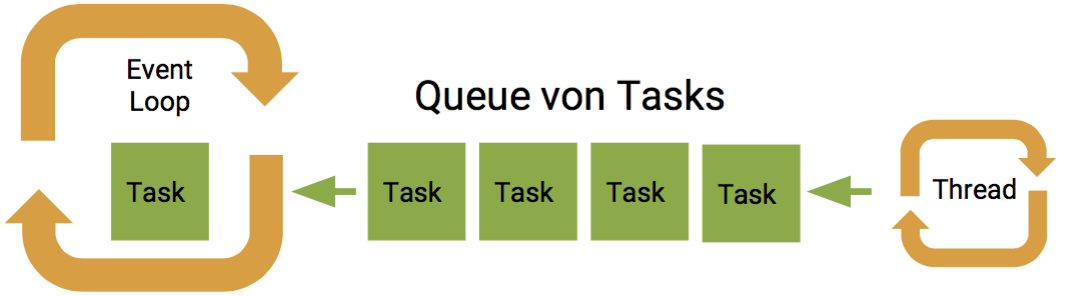
\includegraphics[scale=0.25]{EventLoops.png} \\
Fast alle Listener können mit \code{set[EventName]Listener} registriert werden.
\begin{lstlisting}[language=java]
button.setOnClickListener(new View.OnClickListener() {
  @Override
  public void onClick(View v) {
    /* ... */
  }
});
\end{lstlisting}
Oder onClick Listener in XML deklariert
\begin{lstlisting}[language=xml]
android:onClick="onButtonClicked"
\end{lstlisting}
Alternativ zur anonymen Klasse, kann die Activity auch das Interface implementieren, das kann man mit  (\code{setOnClickListener(this))} bekannt machen.

Ein Listener lässt sich auch bei mehreren Views registrieren. Mit dem übergebenen \code{View}-Parameter kann man unterscheiden (Referenz-Vergleich \code{==}) welches Element den Event ausgelöst hat.

\paragraph{TextWatcher}
Bei der Verarbeitung von Texteingaben haben wir mehrere Möglichkeiten auf Events zu reagieren. Das zu implementierene Interface (\code{TextWatcher}) umfasst 3 Methoden:
\begin{itemize}
\item \code{beforeTextChanged}: Wird aufgerufen bevor der Text geändert wird
\item \code{onTextChanged}: Wird aufgerufen sobald der Text geändert hat
\item \code{afterTextChanged}: Nachdem der Text geändert wurde, kann man den Text noch anpassen (Loop-Gefahr)
\end{itemize}
\begin{lstlisting}[language=java]
editText.addTextChangedListener(new TextWatcher() {
  public void onTextChanged(CharSequence s, int start, int before, int count){ }
  public void beforeTextChanged(CharSequence s, int start, int count, int after){ }
  public void afterTextChanged(Editable s) { }
});
\end{lstlisting}
Bei Eingabefeldern kann man mit \code{setError} Meldungen anzeigen lassen. Dies eignet sich gut für eine Inputvalidierung. Bei jeder Änderung wird diese zurückgesetzt.
\begin{lstlisting}[language=java]
final EditText password = (EditText) findViewById(R.id.password);
password.addTextChangedListener(new TextWatcher() {
  @Override
  public void afterTextChanged(Editable s) {
    String pw = s.toString();
    if (s.length() < 8) {
    password.setError("Passwort muss mindestens 8 Zeichen lang sein.");
    }
  }
  ...
});
\end{lstlisting}
\subsection{Android Testing mit JUnit}
Es gibt mehrere Arten von Tests für eine Activity. Die \code{ActivityUnitTest} manipulieren das UI im Code, die \code{ActivityInstrumentationTestCase2} schickt Clicks und Events an das UI. Um eine App mit mehreren Activities zu testen, gibt es das Espresso Framework, sowie UI Automator um App-übergreifend zu testen.
\begin{lstlisting}[language=java]
public class MainActivityLayoutTest extends ActivityUnitTestCase<MainActivity> {
  public MainActivityLayoutTest() {
    super(MainActivity.class);
  }
  @Override
  protected void setUp() throws Exception {
    super.setUp();
    ContextThemeWrapper context = new
      ContextThemeWrapper(getInstrumentation().getTargetContext(), R.style.AppTheme);
    setActivityContext(context);
    startActivity(
      new Intent(getInstrumentation().getTargetContext(), MainActivity.class),null,null);
}
\end{lstlisting}
Funktionale Tests (ActivityInstrumentationTestCase2) testen eine Activity im echten Systemkontext. Der Test löst Events aus und prüft, ob diese zum erwünschten Resultat führen. Dazu gehören: 
\begin{itemize}
\item Ändert sich das UI wie erwartet
\item Überprüfen von Inputvalidierung
\item Werden Lifecycle Events korrekt behandelt
\end{itemize}
\begin{lstlisting}[language=java]
public class MainActivityInteractionTest extends ActivityInstrumentationTestCase2<MainActivity> {
  public MainActivityInteractionTest() { super(MainActivity.class); }
  public void testSayHi() {
    MainActivity activity = getActivity();
    final EditText editText = (EditText) activity.findViewById(R.id.editText);
    getInstrumentation().runOnMainSync(new Runnable() {
      @Override
      public void run() {
        editText.requestFocus();
      }
    });
    getInstrumentation().waitForIdleSync();
    getInstrumentation().sendStringSync("Hello");
    getInstrumentation().waitForIdleSync();
    Button button = (Button) activity.findViewById(R.id.button);
    TouchUtils.clickView(this, button);
...
\end{lstlisting}

\section{Menüs}
\subsection{Benutzerführung}
Die höchste Klasse jeder XAML App ist die \code{System.Windows.Application}. Diese beinhaltet u.a. ein \code{Current} Property (Singelton) welches statischen Zugriff auf das Application Objekt bietet, das \code{MainWindow}, das Zugriff auf das Hauptfenster bietet und den \code{ShutdownMode} welche das Verhalten beim Programmende definiert.
\paragraph{Current} Das Application Objekt ist als Singelton implentieret. Um es innerhalb der App zu verwenden, muss es oft gecastet werden.
\begin{lstlisting}
public App MyApp => Application.Current as App;
\end{lstlisting}
\paragraph{ShutdownMode} Der ShutdownMode definiert das Verhalten der App beim beenden, davon gibt es 3.
\begin{itemize}
\item \code{OnLastWindowClose}: Dies ist das Standardverhalten, die App beendet sich, sobald das letzte Fenster geschlossen wurde
\item \code{OnMainWindowClose}: Die App wird beendet sobald das Hauptfenster geschlossen wird
\item \code{OnExplicitShutdown}: Die App wird erst beendet, wenn die \code{Shutdown()} Methode aufgerufen wurde.
\end{itemize}
\paragraph{StartupUri} Dies ist der Name der UI Ressource, die beim Start angezeigt werden soll, es ist normalerweise ein \verb+Window+

\paragraph{Startup}

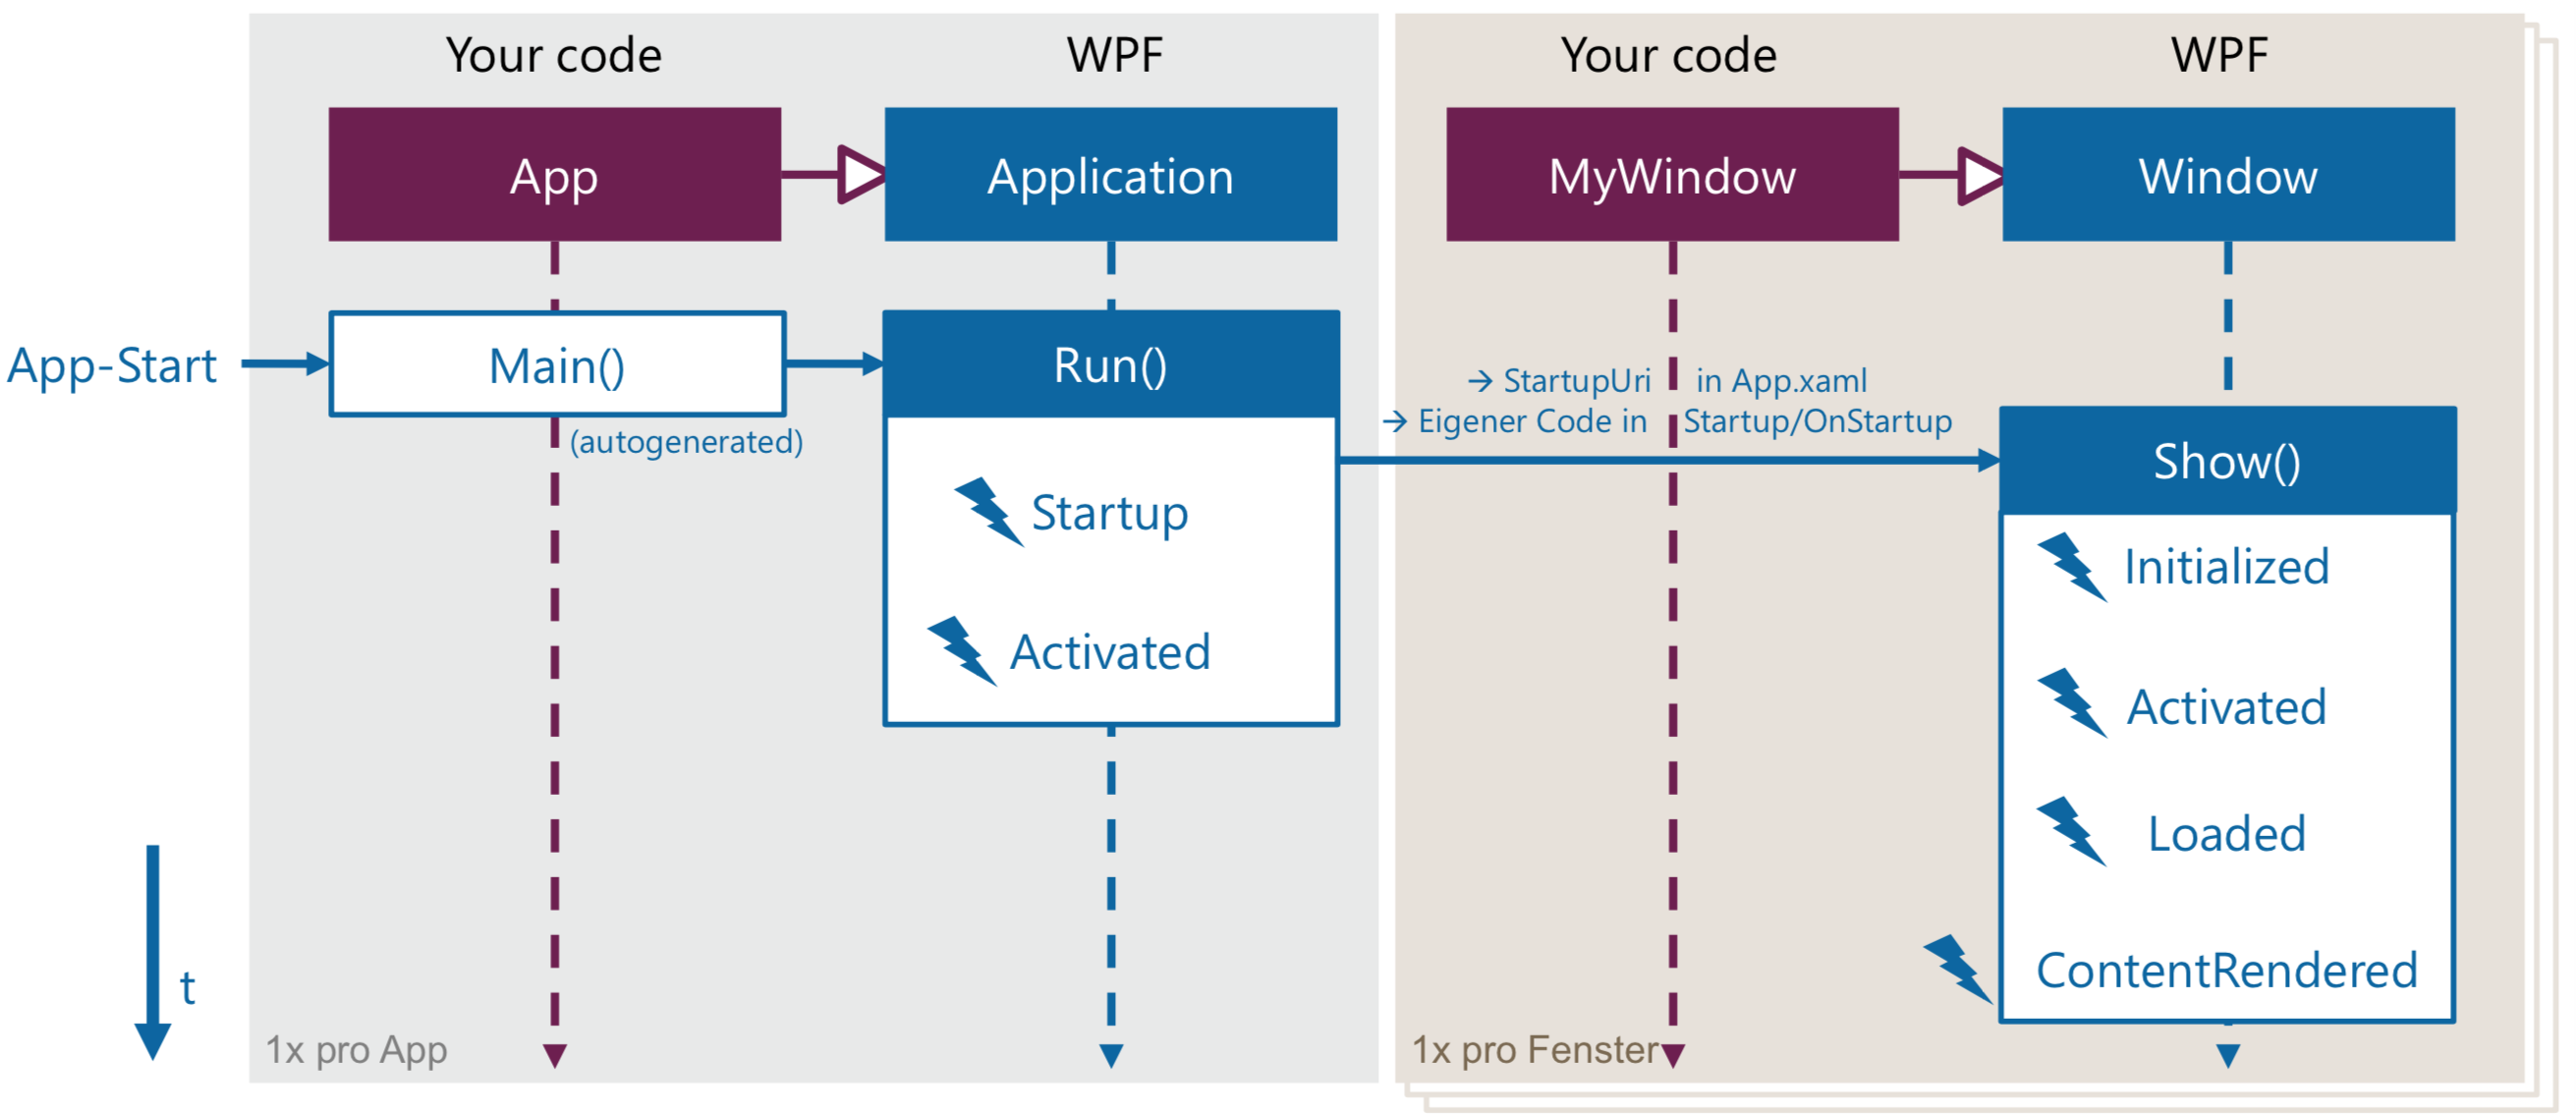
\includegraphics[scale=0.13]{startup.png}

\paragraph{Windows} Das \code{Windows} Property ist eine Liste aller instanziierter Fenster (Window-Objekte) innerhalb der App.
\paragraph{Application-Klasse Methoden} Die \verb+LoadComponent+ Methode lädt eine XAML-Ressource.
\begin{lstlisting}
public static object LoadComponent(Uri uri)
\end{lstlisting}
Der Rückgabetyp muss in den korrekten Typ gecastet werden.\\
Die \verb+FindResouce+ Methode, sucht eine Ressource mit dem angegeben Namen. Es durchsucht App-Ressourcen und System-Ressourcen. Der Rückgabetyp muss ebenfalls in den korrekten Typ gecastet werden.
\begin{lstlisting}
public object FindResource(object resourceKey)
\end{lstlisting}
Die \verb+Shutdown+ Methode beendet die App und gibt optional einen mitgegebenen Exit Code ans System zurück.
\begin{lstlisting}
public void Shutdown([int exitCode])
\end{lstlisting}
\paragraph{Application-Klasse Events}
\begin{itemize}
\item \verb+Activated+: Die App wurde aktivitert (in den Vordergrund geholt)
\item \verb+Deactivated+: Die App wurde deaktiviert
\item \verb+DispatcherUnhandledException+: Eine nicht gefangene Exception ist aufgetreten
\item \verb+Exit+: Die App wird gleich beendet
\item \verb+FragmentNavitation+: Es wurde zu einem bestimmten \verb+NavigationWindow+/\verb+Frame+ navigiert
\item \verb+LoadCompleted+: Aktuelles \verb+NavigationWindow+/\verb+Frame+ wurde vollständig geladen
\item \verb+Navigated+: Aktuelles \verb+NavigationWindow+/\verb+Frame+ wurde gefunden
\item \verb+Navigating+: Navigation zu einem \verb+NavigationWindow+/\verb+Frame+  wurde angefordert
\item \verb+NavigationFailed+: Navigation zu einem \verb+NavigationWindow+/\verb+Frame+ ist fehlgeschlagen
\item \verb+NavigationProgress+: Statusinformation zum Downloadstatus bei Internet-Ressourcen
\item \verb+NavigationStopped+: Ladevorgang des Inhalts der \verb+NavigationWindow+/\verb+Frame+ wurde gestoppt
\item \verb+SessionEnding+: Windows Session wird beendet
\item \verb+Startup+: Die App startet gerade
\end{itemize}
\paragraph{SplashScreen} Es gibt 2 Arten einen SplashScreen zu implementieren. Die automatische Variante ist, ein Bild in das Projekt zu kopieren und bei den FileProperties \verb+BuildAction+ auf SplashScreen zu setzten. Die kontrollierte Variante ist, in der \verb+App_OnStartup+ Methode den SplashScreen zu instanzieren und anzuzeigen.
\begin{lstlisting}
private void App_OnStartup(object sender, StartupEventArgs e)
{
    var screen = new SplashScreen("media/splash.png");
    screen.Show(true);
}
\end{lstlisting}
Der Screen muss dann natürlich auch irgendwann wieder ausgeblendet werden. Alternativ kann man diesen auch nach einer gewissen Zeit ausblenden.
\begin{lstlisting}
private void App_OnStartup(object sender, StartupEventArgs e)
{
    var screen = new SplashScreen("media/splash.png");
    screen.Show(true); // in den Folien steht false
    Thread.Sleep(2000);
    screen.Close(TimeSPan.FromMilliseconds(500));
}
\end{lstlisting}
\subsection{Window Klasse}
Die \verb+Window+ Klasse beschreibt ein Fenster. Sie ist abgeleitet von \verb+ContentControl+ und erlaubt genau 1 Child Element (\verb+LayoutContainer+).
\begin{itemize}
\item \verb+Icon+: Dieses Property beinhaltet eine ICO-Datei, die als Fenster Icon verwendet wird (Ausführbaren Datei und Fensterttitel)
\item \verb+ShowInTaskBar+: Ein Property das angibt, ob das Fenster in der Taskleite angezeigt wird
\item \verb+Topmost+: Zeigt Fenster über allen andern Fenstern der Anwendung an
\item \verb+SizeToContent+: Legt fest, ob die Grösse eines Fensters automatisch an die Grösse des Inhalts angepasst wird.
    \subitem \verb+Manual+: Fenstergrösse anhand Width/Height Angabe(Standart)
    \subitem \verb+Height+: Höhe wird automatisch anhand des Inhalts festgelegt
    \subitem \verb+Width+: Breite wird automatisch anhand des Inhalts festgelegt
    \subitem \verb+WidthAndHeight+: Breite und Höhe werden automatisch anhand des Inhalts festgelegt
\item \verb+ResizeMode+: Gibt an, wie sich die Fenstergrösse ändern darf. Je nach Einstellung werden zusätzlich die Schaltflächen Minimieren/Maximieren im Fenstertitel angezeigt
    \subitem \verb+NoResize+: Fenstergrösse nicht änderbar
    \subitem \verb+CanMinimize+: Fenster kann minimiert und wiederhergestellt werden
    \subitem \verb+CanResize+: Fenstergrösse kann frei verändert werden (Standard)
    \subitem \verb+CanResizeWithGrip+: Wie \verb+CanResize+ aber mit zusätzlichem Resize Grip unten rechts im Fenster
\item \verb+WindowsStartupLocation+: Legt die Postition beim Start fest
    \subitem \verb+CenterOwner+: Fenster wird in Mitte des aufrufenden angezeigt
    \subitem \verb+CenterScreen+: Fenster wird in der Mitte des Bildschirm angezeigt
    \subitem \verb+Manual+: Position wird durch Left/Top Angabe bestimmt (Standart)
\item \verb+WindowState+: Beschreibt die Fensterzustände (Normal, Minimized, Maximized)
\item \verb+WindowStyle+: Gibt den Rahmentyp des Fensters an:
    \subitem \verb+None+: Nur das Client Area ist sichtbar
    \subitem \verb+SingleBorderWindow+: Fenster mit einfachem (dünnem) Rahmen
    \subitem \verb+ThreeDBorderWindow+: Fenster mit 3D Rahmen
    \subitem \verb+ToolWindow+: Verankertes Tool-Fenster
\end{itemize}
\paragraph{Window-Klasse Methoden}
\begin{itemize}
\item \verb+Activate+: Fenster aktivieren
\item \verb+Close+: Fenster schliessen
\item \verb+DragMove+: Ermöglich das Verschieben des Fensters, falls die linke Maustaste gedrückt ist
\item \verb+GetWindow+: Statische Methode, ruft das Root-Window Objekt zum Control ab (DI)
\item \verb+Hide+: Macht das Fenster unsichtbar
\item \verb+Show+: Zeigt das Fenster an
\item \verb+ShowDialog+: Zeigt das Fenster an und blockiert, bis das Fenster geschlossen wird
\end{itemize}
\paragraph{Window-Klasse Events}
\begin{itemize}
\item \verb+Activated+: Fenster wurde aktiviert
\item \verb+Closed+: Fenster wurde geschlossen
\item \verb+Closing+: Fenster wird gleich geschlossen
\item \verb+ContentRendered+: Fensterinhalt wurde gezeichnet
\item \verb+Deactivated+: Fenster wurde deaktiviert
\item \verb+LocationChanged+: Position des Fensters wurde geändert
\item \verb+StateChanged+: WindowState hat geändert
\end{itemize}
\subsection{Dialogfenster} 
Dialogfenster dienen zum Abruf von Daten und sind meist Modal (blockierend). \\
Ein Dialogfenster wird mit der Methode \verb+ShowDialog+ angezeigt. Im Dialogfenster kann die Property DialogResult gesetzt werden (boolean). Sobald dies gesetzt wurde wird das Dialogfenster geschlossen. 
\begin{lstlisting}[language=xml]
<Button Content="Cancel" IsCancel="true" />
<Button Name="OkButton" Content="OK" IsDefault="true" Click="OkButton_OnClick" />
\end{lstlisting}
Das \verb+IsCancel+ Property schliesst bei \verb+true+ das Dialogfenster automatisch (kein Event-Handling).
\begin{lstlisting}
private void OkButton_OnClick(object sender, ReoutedEventargs e)
{
    SelectedCustomer = "MaxMuster";
    // trigger dialog close as side effect
    DialogResult = true; 
}
\end{lstlisting}
\paragraph{Fenster mit Spezialformen} Die Fensterrahmen können mittels Clipping verändert werden. Das setzt jedoch folgende Fenstereigenschaften voraus:
\begin{itemize}
\item \verb+AllowsTransparency=true+
\item \verb+WindowStyle=none+
\item \verb+ResizeMode=NoResize+
\end{itemize}
Man kann die Form in \verb+Window.Clip+ mittels einem Geometry-Element festlegen
\begin{lstlisting}[language=xml]
<!-- Rechteck mit abgerundeten Raendern -->
<Window.Clip>
    <RectangleGeometry RadiusX="8" RadiusY="8" Rect="0,0,800,600" />
</Window.Clip>
\end{lstlisting}
\subsection{Menu}
Die Menüs sind herkömmliche Windows-Menüs und werden üblicherweise am oberen Fensterrand angedockt. Mit dem Property \verb+IsMainMenu=true+ kann man das Menü standartmässig als Hauptmenü definieren.
\paragraph{MenuItem} MenuItems sind beliebig verschachtelbar. Sie haben ein \verb+Header+ als anzuzeigenden Texts (Underscore = Accelerator-Key), \verb+IsCheckable+ definiert, ob der Eintrag ein Zustand ist (mit \verb+IsChecked+ kann Zustand gesetzt bzw. geprüft werden). Das \verb+InputGestureText+ Property definiert, definiert einen Text, der im MenuItem rechtsbündig angezeigt wird (Shortcuts wie Ctrl+V), um zu Funktionieren müssen diese noch behandelt werden, beispielsweise mit Commands.
\begin{lstlisting}[language=xml]
<Menu DockPanel.Dock="Top">
    <MenuItem Header="_File">
        <MenuItem Header="_Recent">
            <MenuItem Header="Secret.txt" />
            <MenuItem Header="TopSecret.txt" />
        </MenuItem>
        <Separator />
        <MenuItem Header="E_xit" InputGestureText="CTRL + Q" />
    </MenuItem>
    <MenuItem Header="_Edit">
        <MenuItem Header="_Cut" InputGestureText="CTRL + X" />
        <MenuItem Header="C_opy" InputGestureText="CTRL + C" />
        <MenuItem Header="_Paste" InputGestureText="CTRL + V" />
        <Separator />
        <MenuItem Header="_Settings">
            <MenuItem Header="_Always On Top" IsChecked="True"></MenuItem>
            <MenuItem Header="_Modern UI" IsChecked="false"></MenuItem>
        </MenuItem>
    </MenuItem>
</Menu>
\end{lstlisting}
\paragraph{Kontextmenus} Das \verb+ContextMenu+ stellt ein kontextspezifisches Menü zur verfügung. Es funktioniert wie das Menü und kann direkt mit der Property-Syntax für ein Control erstellt werden.
\begin{lstlisting}[language=xml]
<Button.ContextMenu>
    <ContextMenu>
        <MenuItem Header="Hilfe" />
        <MenuItem Header="Fehler melden" />
    </ContextMenu>
</Button.ContextMenu>
\end{lstlisting}
\paragraph{StatusBar} Die Statusbar dient zur Anzeige von zusätzlichen Informationen (meist am unteren Fensterrand). Es ist ein Container, ähnlich wie beim DockPanel, dabei füllt das letzte Element die ganze restliche Breite.
\begin{lstlisting}[language=xml]
<StatusBar DockPanel.Dock="Bottom">
    <StatusBarItem Width="150">Press CTRL + Q to quit</StatusBarItem>
    <Separator />
    <StatusBarItem>Ready</StatusBarItem>
</StatusBar>
\end{lstlisting}
Für Kontextbezogene Statusinformationen können \verb+StatusBarItem+ Elemente benannt werden und dann programmatisch darauf zugegriffen werden, oder man arbeitet mit Databinding.
\paragraph{Toolbar} kann entweder ein \verb+ToolBarTray+ sein, der als Container für Toolbars dient, oder ein \verb+Toolbar+ der als Container für Toolbar-Buttons und sonstige Toolbar-Controls dient. Die ToolBarTray ermöglicht das Verschieben und Umgruppieren der Toolbars und ist typischerweise angedockt. \\
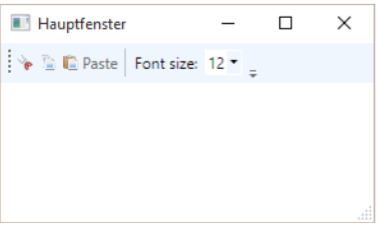
\includegraphics[scale=0.40]{Toolbar.png}
\begin{lstlisting}[language=xml]
<ToolBarTray DockPanel.Dock="Top">
    <ToolBar>
        <Button Command="Cut" ToolTip="...">
            <Image Source="/media/clip_cut.png" Width="12" Height="12" />
        </Button>
    <Button Command="Copy" ToolTip="Copy selection to Windows Clipboard.">
        <Image Source="/media/clip_copy.png" Width="12" Height="12" />
    </Button>
    <Button Command="Paste" ToolTip="Paste from Windows Clipboard.">
        <StackPanel Orientation="Horizontal">
            <Image Source="/media/clip_paste.png" Width="12" Height="12" />
            <TextBlock Margin="3,0,0,0">Paste</TextBlock>
        </StackPanel>
    </Button>
    <Separator />
    <Label>Font size:</Label>
    <ComboBox>
        <ComboBoxItem>10</ComboBoxItem>
        <ComboBoxItem IsSelected="True">12</ComboBoxItem>
        <ComboBoxItem>14</ComboBoxItem>
        <ComboBoxItem>16</ComboBoxItem>
    </ComboBox>
    </ToolBar>
</ToolBarTray>
\end{lstlisting}
\paragraph{Ribbon} Das Ribbon ist seit Office 2007 bekannt und ist seither immer stärker verbreitet. 
\begin{lstlisting}[language=xml]
<Ribbon Name="Ribbon">
    <Ribbon.ApplicationMenu>
        <RibbonApplicationMenu SmallImageSource="media/home.png">
            <RibbonApplicationMenuItem Header="Hello _Ribbon"
                Name="MenuItem1"
                ImageSource="media/home.png"/>
        </RibbonApplicationMenu>
    </Ribbon.ApplicationMenu>
    <RibbonTab x:Name="HomeTab" Header="Start">
        <RibbonGroup x:Name="Clipboard" Header="Clipboard">
            <RibbonButton x:Name="Button1" Label="Paste"
                LargeImageSource="media/clip_paste.png" />
            <RibbonButton x:Name="Button2" Label="Cut"
                SmallImageSource="media/clip_cut.png" />
            <RibbonButton x:Name="Button3" Label="Copy"
                SmallImageSource="media/clip_copy.png" />
        </RibbonGroup>
    </RibbonTab>
</Ribbon>
\end{lstlisting}
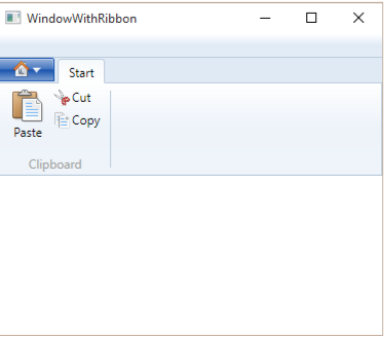
\includegraphics[scale=0.35]{Ribbon.png}
\section{Commands} bieten eine Alternative zum Event. Commands müssen nicht abgefangen und behandelt werden, sie werden durch die Control selbst aufgerufen. Es ist eine standartisierte Ausführung eines Befehls und ermöglicht die Wiederverwendung derselben Aktion. Eine Command-Methode muss \verb+RoutedUICommand+ als Rückgabetyp haben und statisch sein.
\begin{lstlisting}
public static RoutedUICommand MyCutCommand = new RoutedUICommand(
    "Ausschneiden",
    "MyCut",
    typeOf(WindowWithToolbar)
);
\end{lstlisting}
Der \verb+RoutedUICommand+ nimmt auch noch einen 4. Paramter entgegen, in dem man \verb+InputGestures+ entweder einzeln oder als \verb+InputGestureCollection+ mitgeben kann.
\begin{lstlisting}[language=xml]
<MenuItem Header="_Cut" InputGestureText="CTRL + X" Command="local:WindowWithToolbar.MyCutCommand" />
\end{lstlisting}
Commands können auch an Event-Handler gebunden werden und Shortcuts definiert werden.
\begin{lstlisting}[language=xml]
<!-- Binding an Event -->
<Window.CommandBindings>
    <CommandBinding Command="local:WindowWithToolbar.MyCutCommand" Executed="MyCutCommand_Executed" />
</Window.CommandBindings>
<!-- Shortcut definieren -->
<Window.InputBindings>
    <KeyBinding Key="X" Modifiers="Control" Command="local:WindowWithToolbar.MyCutCommand" />
</Window.InputBindings>
\end{lstlisting}
Im Code-Behind kann dann wie gewohnt ein Handler definiert werden.
\begin{lstlisting}
public void MyCutCommand_Executed(object sender, ExecutedRoutedEventArgs e){ ... }
\end{lstlisting}
\section{Automated UI Testing}
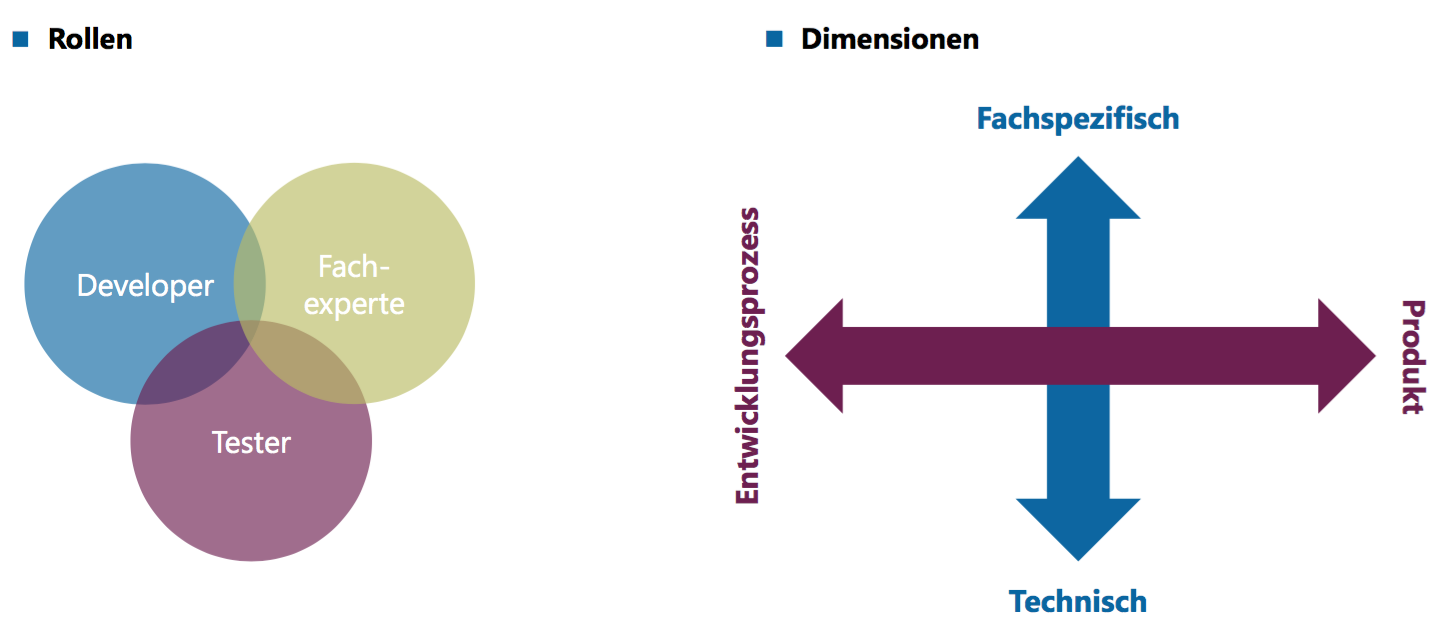
\includegraphics[scale=0.25]{Testing1.png}
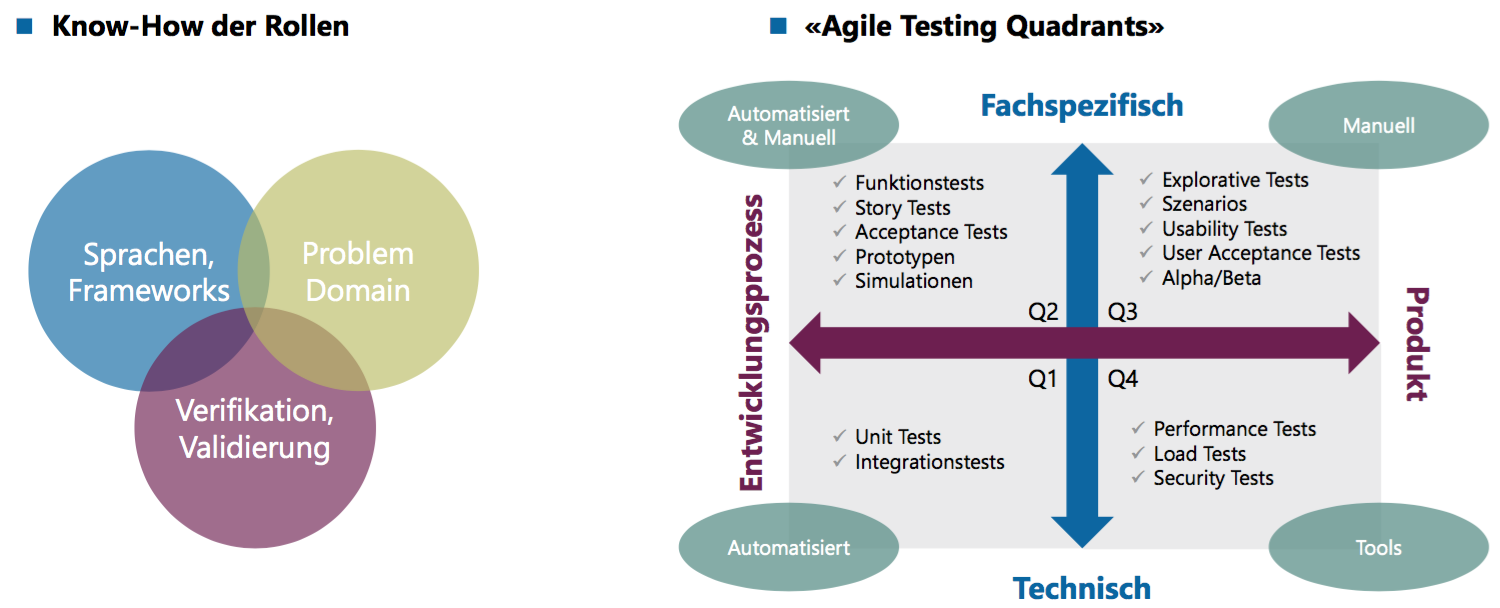
\includegraphics[scale=0.25]{Testing2.png}
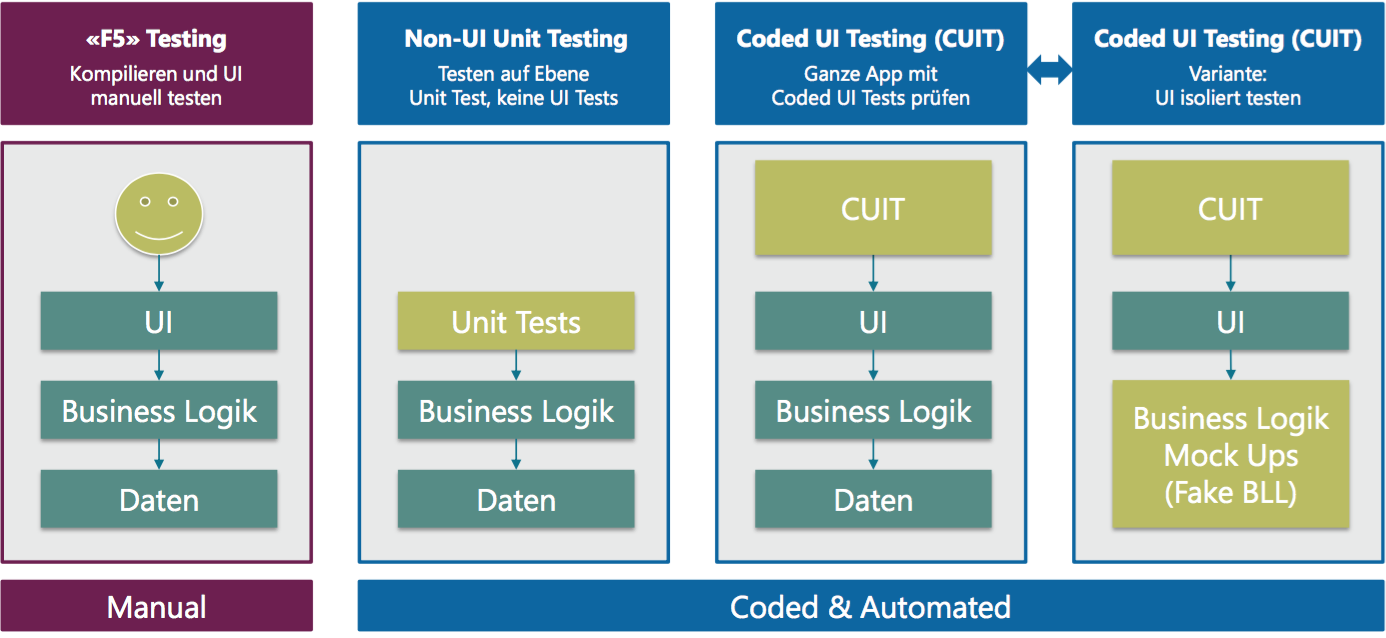
\includegraphics[scale=0.25]{Testing3.png} \\
Es gibt 4 Varianten UIs zu testen. Das \textbf{Non-UI Unit Testing} Test auf Code Ebene (normale Unit-Tests) und führt keine UI-Tests durch. Das \textbf{Coded UI Testing (CUIT)} testet die ganze App mit Coded UI Tests. Diese Variante kann man auch mit isolierten UI Komponenten durchführen, welche dann aber Fake Komponenten benötigen (die 4. Variante ist das F5-Testing, der Benutzer testet die App gleich selbst).
\subsection{TestStack}
Der TestStack ist eine Sammlung von OpenSource Projekten um Tests in .NET Projekten zu automatisieren. Dazu gehört das \textbf{TestStack.White} Framework. Es ist ein CUIT-FW für WPF und basiert auf Microsofts UI Automation Framework. \\
Als Vorbereitung muss man eine Testklasse erstellen.
\begin{lstlisting}
[TestClass]
public class MyUiTest
{
    [TestMethod]
    public void MyUiTestMethod(){ ... }
}
\end{lstlisting}
Danach muss man das Verzeichnis mit der WPF App Assembly festlegen. Dies kann dann als Read-Only Property in der Testklasse hinzugefügt werden.
\begin{lstlisting}
// Directory in which tests are running
public string BaseDir => Path.GetDirectoryName(Assembly.GetExecutingAssembly().Location);
// System under test
public string SutPath => Path.Combine(BaseDir, ${nameof(MenusAndCommands)}.exe);
//$
\end{lstlisting}
Nun kann man die Tests entwickeln. \\
Zuerst neues Application Objekt aus dem WPF App Assembly erstellen:
\begin{lstlisting}[caption="Neues Application Objekt aus dem WPF App Assembly erstellen"]
var app = Application.Launch(SutPath);
\end{lstlisting}
Die Variable enthät ein UI-Automatisierungsobjekt des Typs \verb+TestStack.Whie.Application+.
Danach kann man die Fenster abrufen:
\begin{lstlisting}
// Mit Fenstertitel abrufen
var window = app.GetWindow("Hauptfenster", InitializeOption.NoCache);
// Aus Liste der Fenster abrufen
var window = app.GetWindows.First();
// Anhand der ID(Name-Attribut) abrufen
var window = app.getWindow(SearchCriteria.ByAutomationId"(Win1"), InitializeOption.NoCache);
\end{lstlisting}
Die Variable \verb+window+ enthäht nun ein UI-Automatisierungsobjekt des Typs \verb+TestStack.White.UIItems.WindoItems.Window+.\\
Danach muss man die Controls abrufen:
\begin{lstlisting}
// Anhand Beschriftung abrufen
var button = window.Get<Button>(SearchCriteria.ByText("Speichern"));
// Anhand ID(Name-Attribut) abrufen
var button window.Get<Button>("SaveButton");
\end{lstlisting}
Die Variable \verb+button+ enthält nun ein UI-Automatisierungsobjekt des Typs \verb+TestStack.White.UIItems.Button+.\\
Schlussendlich können Aktionen ausgeführt werden:
\begin{lstlisting}
Assert.AreEqual("Speichern", button.Text);
button.Click();
Assert.AreEqual("Gespeichert!", button.Text);
\end{lstlisting}
\begin{lstlisting}
var input = window.Get<TextBox>("NameInput");
Assert.IsTrue(string.IsNullOrEmpty(input.Text));
var newText = "You've been hacked!";
input.Text = newText;
Assert.AreEqual(newText, input.Text);
\end{lstlisting}
Schlussendlich muss die App noch mittels \verb+app.Close()+ beendet werden.\\
Mit \verb+Desktop.CaptureScreenshot()+ erhält man ein Bitmap Objekt mit einem Bild des aktuellen Bildschirms.
\begin{lstlisting}
var screenshot = Desktop.CaptureScreenshot();
var path = System.IO.Path.Combine(BaseDir, "screenshot.png");
screenshot.Save(path, ImageFormant.Png);
\end{lstlisting}


\section{GUI Design}
\subsection{WPF Ressourcen}
Mit WPF Ressourcen kann man nützliche Objekte (Brushes, Styles, Templates etc.) zentral definieren und wiederverwenden.
\subsection{Resources}
\paragraph{Physikalische Ressourcen} In den File Properties kann man eine Datei als WPF-Ressource deklarieren welche dann in die Binärdatei einkompiliert werden. Zugegriffen kann dann mittels Resource-Key (relativer Pfadname).
\paragraph{Resource} Jedes beliebige Objekt in XAML kann als Ressource definiert werden. Es bird mit einem Key-Attribut und dem x-Namespace benannt.
\begin{lstlisting}[language=xml]
<Application.Resources>
    <SolidColorBrush x:Key ="MyButtonBackground" Color="#EEEEEE" />
</Application.Resources>
\end{lstlisting}
Unter diesem Key sind Ressourcen dann auch ansprechbar
\begin{lstlisting}[language=xml]
<Button Background="{StaticResource MyButtonBackground}" Content="Save" />
\end{lstlisting}
\paragraph{ResourceDictionary} Ist ein Behälter um Ressourcen zu speichern. Es indexiert nach dem Ressourcen-Namen (\verb+x:Key+) und kann in allen Elementen, welche von FrameworkElement ableiten, verwendet werden. Wenn auf eine Ressource zugegriffen werden möchte, wird \begin{enumerate*}[label=\itshape \arabic*\upshape.]\item Key im Element und allen Parent-Nodes gesucht (Logical Tree), \item dann wird der Key in \verb+Application.Resources+ gesucht, \item als letztes wird in System-Ressourcen gesucht.\end{enumerate*}. Die Reheinfolge im XAML-Code ist wichtig.
\paragraph{System Ressources} Auf Ressourcen in Namespace \verb+System.Windows+ kann man mittels statischer Properties zugegriffen werden. Dazu gehören: \verb+SystemColors+, \verb+SystemFonts+ und \verb+SystemParamters+.
\begin{lstlisting}[language=xml]
StaticResource="{StaticResource[name]}"
\end{lstlisting}
Die Statische Bindung macht CompileTime Check und findet Fehler früh.
\begin{lstlisting}[language=xml]
DynamicResource="{DynamicResource[name]}"
\end{lstlisting}
Anstelle von \verb+[name]+ steht der Key der Ressource
In der Dynamische Bindung wird ein RuntimeCheck gemacht und lässt dynamisch erzeugte und geladene Ressourcen zu. Beim Static Binding wird bei Objektkonstruktion ausgewertet, beim Dynamic Binding einmal pro Zugriff.
\paragraph{FindResource} Mit der Methode \verb+FrameworkElement.FindResources+  können Zugriffe auf XAML Resourcen gemacht werden.
\begin{lstlisting}
var okText = (string)FindResource("OkText");
var bgBrush = FindResource("DarkBrush") as Brush;
\end{lstlisting}

\subsubsection{Zugriff}

\begin{enumerate}
    \item Key wird im Element und in allen Parent-Nodes gesucht.
    \item Key wird in Application.Resources gesucht.
    \item Key wird in System-Ressourcen gesucht.
\end{enumerate}


\section{Data Trigger}
(in \code{Style.Triggers} eingebunden, wie vorher. Beispiel: Style ist für ListBoxItem, rote Schrift wenn nicht mehr an Lager (\code{InStock == 0})
\begin{lstlisting}
<DataTrigger Binding="{Binding InStock}" Value="0">
    <Setter Property="Foreground" Value="Red" />
</DataTrigger>
\end{lstlisting}

\section{Visual State Manager}

Ermöglicht innerhalb eines ControlTemplate-Elements unterschiedliche Darstellungen anhand eines Zustands.

Wurde erst später (nach Triggern) eingeführt => mit Silverlight => Nicht weiter Besprochen.

\section{Styles}

\begin{lstlisting}
<!-- App.xaml -->
<Application x:Class="ModernUi.App"
             xmlns="http://schemas.microsoft.com/winfx/2006/xaml/presentation"
             xmlns:x="http://schemas.microsoft.com/winfx/2006/xaml"
             xmlns:local="clr-namespace:ModernUi"
             StartupUri="MainWindow.xaml">
    <Application.Resources>
        <ResourceDictionary Source="style.xaml"></ResourceDictionary>
    </Application.Resources>
</Application>

<!-- Style.xaml -->
<Window.Resources>
    <!-- benannten Style als Basis benutzen -->
    <Style x:Key="DefaultButtonStyle" TargetType="Button">
      <Setter Property="BorderThickness" Value="1" />
      <Setter Property="BorderBrush" Value="Black" />
      <Setter Property="Background" Value="Transparent" />
      <Setter Property="Foreground" Value="Black" />
      <Setter Property="FontFamily" Value="Segoe UI" />
      <Setter Property="Margin" Value="2" />
      <Setter Property="Padding" Value="10 2 10 2" />
      <Setter Property="FontSize" Value="13" />
    </Style>
    <!-- Den obigen benannten Style erben und auf alle Buttons anwenden -->
    <Style TargetType="Button" BasedOn="{StaticResource DefaultButtonStyle}"> </Style>
    <!-- für den Help Button noch einen abgeleiteten Style definieren --> <Style x:Key="MyHelpButtonStyle" TargetType="Button"
           BasedOn="{StaticResource DefaultButtonStyle}">
      <Setter Property="Foreground" Value="Gray" />
      <Setter Property="BorderBrush" Value="Gray" />
    </Style>
</Window.Resources>

<!-- Window.xaml -->
<GradientStop Offset="0" Color="{StaticResource BaseColor}" />
\end{lstlisting}

\subsubsection{explizit}
\begin{lstlisting}
<Style x:Key="MyButtonStyle">
    <Setter Property="Button.Foreground" Value="#000000" />
    <Setter Property="Button.Background" Value="#FFFFFF" />
    <!-- auch komplexes möglich -->
    <Setter Property="Button.Background">
        <Setter.Value>
            <LinearGradientBrush StartPoint="0,0" EndPoint="0,1">
                <GradientStop Offset="0" Color="#dddddd"></GradientStop>
                <GradientStop Offset="0.5" Color="#F0F0F0"></GradientStop>
                <GradientStop Offset="1" Color="#dddddd"></GradientStop>
            </LinearGradientBrush>
        </Setter.Value>
    </Setter>
</Style>
\end{lstlisting}

Verwenden mit:\\\code{<Button Style="{StaticResource MyButtonStyle}" Content="Cancel" />}

\subsubsection{implizite Styles}
Man kann auch einen \code{TargetType="Button"} einfügen. Der Klassenname (\code{Button.Foreground}) kann dann weggelassen werden (\code{Foreground}).

Lässt man den Key weg, gilt der Style für alle Elemente des Controls

Man kann auch ableiten, mit \code{BasedOn={StaticResource MyButtonStyle}}.

Möchte man aber den Grundstil als Standard-Stil haben, muss man einen Sentinel einfügen, der den Key weglässt und nur BasedOn ist (der Grundstil muss einen Key haben, damit man davon ableiten kann)

\begin{lstlisting}[language=xml]
<Style TargetType="Button" x:Key="BaseButton"><!--Nutzung über Key-->
    <!-- verschiedene Setter -->
</Style>
<!-- Sentinel, gilt für alle Button -->
<Style TargetType="Button" BasedOn="{StaticResource BaseButton}" />
<!-- spezifischer Stil, Nutzung über Key -->
<Style TargetType="Button" x:Key="DisabledButton" 
    BasedOn="{StaticResource BaseButton}">
    <!-- verschiedene Setter -->
</Style>
\end{lstlisting}

Es gibt aber auch einen einfacheren Weg:
\begin{itemize}
    \item Default-Style belassen (TargetType ja, aber ohne ID)
    \item Sentinel-Style weglassen
    \item abgeleiteter Stil: \code{BasedOn="{StaticResource {x:Type Button}}"}
\end{itemize}

\begin{lstlisting}[language=xml]
<Style TargetType="Button"><!--Nutzung über Key-->
    <!-- verschiedene Setter -->
</Style>
<!-- spezifischer Stil, Nutzung über Key -->
<Style TargetType="Button" x:Key="DisabledButton" 
    BasedOn="{StaticResource {x:Type Button}}">
    <!-- verschiedene Setter -->
</Style>
\end{lstlisting}
\section{Umgang mit Daten}
Ein grosses Feature von WPF ist das DataBinding. 
\paragraph{Markup Extensions}
\begin{itemize}
\item \verb+{x:Type [Datentyp]}+: Liefert angegebene Klasse
\item \verb+{x:Static [Pfade]}+: Bindet eine Konstante, statische Property, Feld oder Enum
\item \verb+{x:Null}+: Null Wert
\item \verb+{StaticResource [Name]}+: Statische Bindung an Ressource
\item \verb+{DynamicResource [Name]}+: Dynamische Bindung an Ressource
\item \verb+{Binding ...}+: Data Binding Ausdruck
\item \verb+{RelativeSource ... }+: Setzt die Data Binding Source auf eine relevanten Bezug im Logical Tree
\item \verb+{TemplateBinding ...}+: Bindet Wert an Eigenschaft des mittels Template dargestellten Controls
\item \verb+{x:Reference ...}+: Abk. für \verb+{Binding Elementname=...}+
\end{itemize}
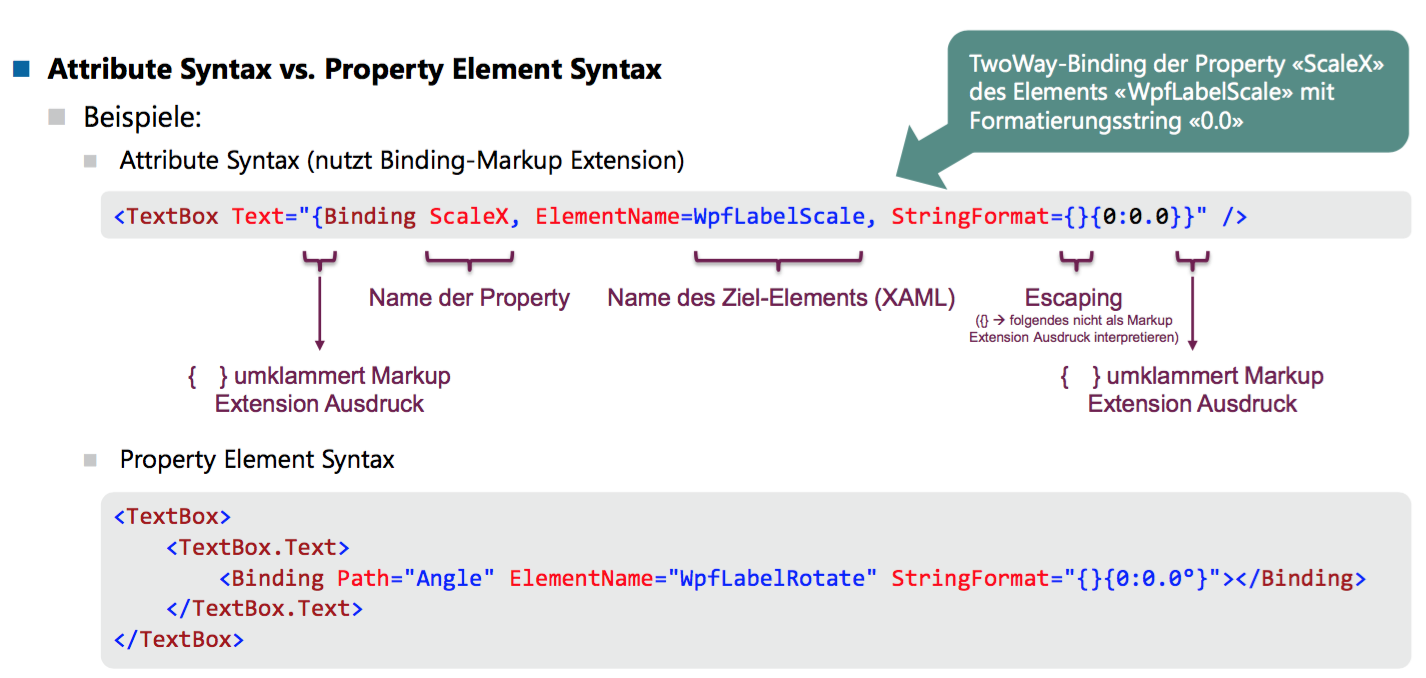
\includegraphics[scale=0.25]{DataBinding.png}
\subsection{Überblick DataBinding}
\paragraph{Binding Base}
\begin{itemize}
\item \verb+Delay+: Verzögerung in Millisekunden zwischen DataBinding Operation
\item \verb+FallbackValue+: Standardwert, falls Data Binding nicht funktioniert
\item \verb+StringFormat+: Formatierungsangabe für die Umwandlung des Quellwertes in einen String
\item \verb+TargetNullValue+: Standardwert, falls Quellwert == null
\end{itemize}
\paragraph{Binding}
\begin{itemize}
    \item \verb+BindsDirectlyToSource+: Soll Angabe der Path-Property relativ zum aktuellen Datenprovider (\verb+true+) oder relativ zum Datenkontext (\verb+false+) ausgewertet werden (Nur selten sinnvoll)
    \item \verb+Converter+: Converter der beim Binding benutzt werden soll
    \item \verb+ConverterCulture+: Länderspezifische Einstellungen (\verb+CultureInfo+), welche beim Konvertieren benutzt werden soll
    \item \verb+ConverterParameter+: Zusätzlicher Parameterwert, der dem Converter übergeben werden soll
    \item \verb+ElementName+: Name des XAML-Elements auf welches gebunden werden soll
    \item \verb+Mode+: Richtung des DataBinding (OneTime, OneWay, TwoWay, OneWayToSource)
    \item \verb+Path+: Pfad zur Datenquelle, Objektpfadsyntax
    \item \verb+XPath+: XPath Ausdruck zum Zugriff auf eine XML Datenquelle
    \item \verb+RelativeSource+: Setzt Datenquelle auf Objekt relative zum Ort des aktuellen Elements
    \item \verb+Source+: Setzt Datenquelle
    \item \verb+UpdateSourceTrigger+: Zeitpunkt zu welchem DataBinding getriggert wird
        \subitem Default: Nutzt festgelegte Trigger der Ziel Property
        \subitem Explicit: Nur beim expliziten Aufruf von \verb+UpdateSource()+
        \subitem LostFocus: Fokusverlust des Elements
        \subitem PropertyChanged: Bei jeder änderung des Inhalts
\end{itemize}

\subsection{DataContext, Source, RelativeSource}
Die Datenquelle ist standartmässig nicht gesetzt, muss also explizit gesetzt werden. 
\paragraph{DataContext} Jedes Element, das von \verb+FrameworkElement+ ableitet, besitzt diese Property. Diese wird Standartmässig von DataBinding als Quelle genutzt und ist ebenfalls in Child-Controls gültig. Diese Property wird im Code-Behind, meist auf Ebene der Fenster, gesetzt.
\paragraph{Source} Ermöglicht die Angabe der Datenquelle direkt im DataBinding Ausdruck. Dieses Property kann auf Ressourcen (Static/Dynamic) oder statische (Static) binden.
\paragraph{RelativeSource} Ermöglicht die Angabe einer relativen Datenquelle im Visual Tree. Es gibt eine eigene Markup Extension dafür. Mit dem Property \verb+Mode+ gibt man den Suchmodus an. Modi dafür sind: \verb+FindAncestor+(Sucht übergeordnetes Element des Typs), \verb+PreviousData+ (Bindet auf das vorhergehende Element, bsp: Delta Vergleiche), \verb+Self+ (Bindet auf das Element selbst), \verb+TemplatedParent+ (Bindet auf Element, für welches Control Template gilt, sinnvoll innerhalb Template). Das Property \verb+AncestorLevel+ Gibt die Vorgänger-Position an und der \verb+AncestorType+ ist der Typ des zu suchenden Vorgänger-Elements.
\begin{lstlisting}[language=xml]
<Label Content="{Binding RelativeSource={RelativeSource FindAncestor, AncestorType=Window}, Path=Title}" />
\end{lstlisting}
\paragraph{Path} Ist die Standart-Property eines Binding-Ausdrucks. Dieser kann deshalb weggelassen werden (\verb+{Binding Firstname}+ ist dasselbe wie \verb+{Binding Path=Firstname}+). Für die Angabe der zu bindenden Property kann auch Objektsyntax verwendet werden (auch Array Syntax ist erlaubt).
\subsection{Converter}
\paragraph{IValueConverter} Ein Interface welches alle Converter implementieren müssen
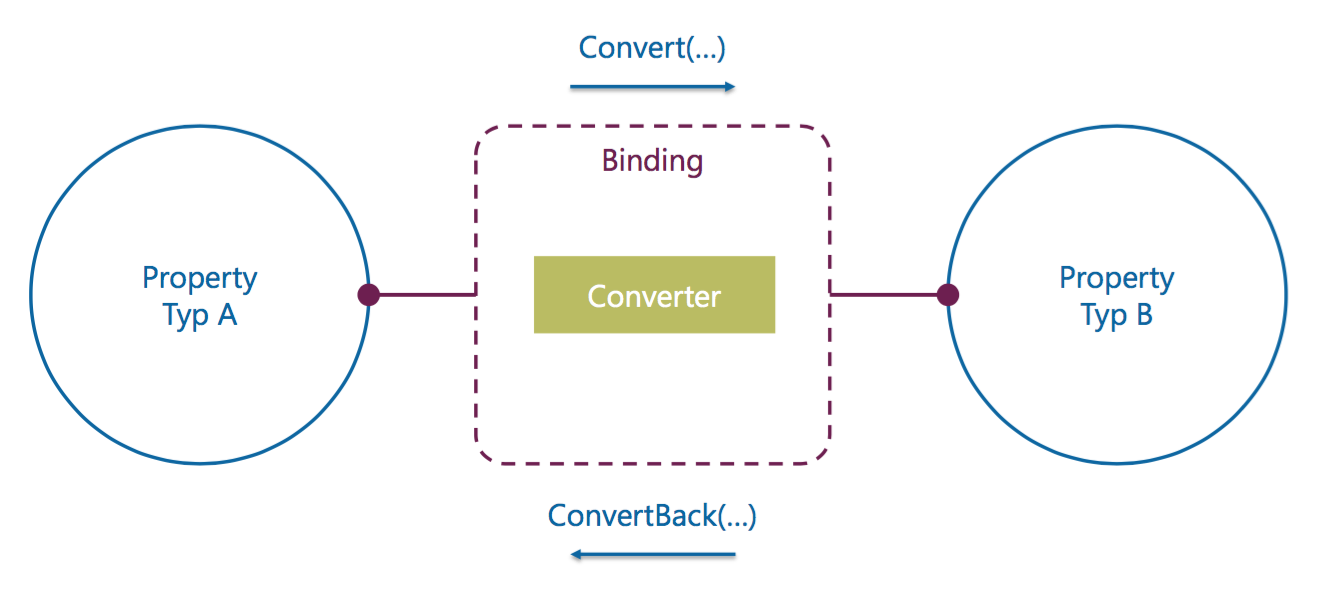
\includegraphics[scale=0.25]{IValueConverter.png}

Es ist auch möglich, nur eine der Methoden zu überschreiben und die andere mit NotImplementedException auszustatten, wenn man es selber nicht verwendet

\begin{lstlisting}[caption="Konvertiert bool oder Nullable in Visibility und zurück"]
public sealed class BooleanToVisibilityConverter: IValueConverter
{
    // value = bool oder nullable, targetType = Visibility
    public object Convert(object value, Type targetType, object parameter, CultureInfo culture)
    {
        return value is bool && (bool)value == true ? Visibility.Visible : Visibility.Collapsed;
    }
    // value = Visibility value, targetType = bool
    public object ConvertBack(object value, Type targetType, object parameter, CultureInfo culture)
    {
        return value as Visibility? == Visibility.Visible
    }
}
\end{lstlisting}
\paragraph{IMultiValueConverter} Das Interface dass alle MultiConverter implementieren müssen.
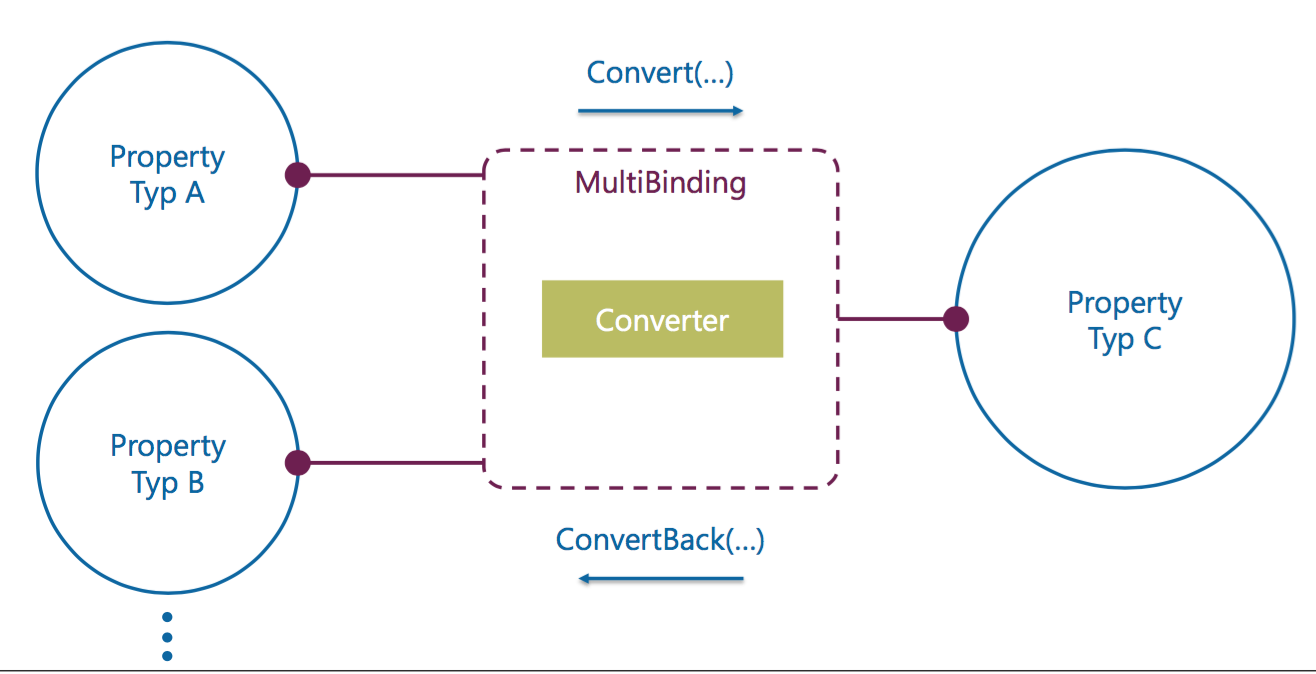
\includegraphics[scale=0.25]{IMultiValueConverter.png}
\begin{lstlisting}
public class RgbToColorConverter: IMultiValueConverter
{
    public object Convert(object[] values, Type targetType, object paramter, CultureInfo culture)
    {
        if (values == null)
            return DependencyProperties.Unsetvalue;
        if(values.Length != 3)
            throw new NotSupportedException("3 Values needed)";
        var r = (byte)System.Convert.ToInt32(values[0]);
        var g = (byte)System.Convert.ToInt32(values[1]);
        var b = (byte)System.Convert.ToInt32(values[2]);
        return Color.FromRgb(r,g,b);
    }
    public object[] ConvertBack(object value, Type[] targetType, object parameter, CultureInfo culture)
    {
        if(value == DependencyProperty.UnsetValue)
            return null;
        if(value is Color)
        {
            var color = (Color) value;
            var colors = new object[] {color.R, color.G, color.B};
            return colors;
        }
        return null;
    }
}
\end{lstlisting}
\paragraph{Value Converter anwenden} Um einen Converter anwenden zu können wird eine Instanz benötigt. Instanziierung:
\begin{lstlisting}[language=xml, caption="Instanzieren"]
<Window.Resources>
    <local:RgbToColorConverter x:Key="MyRgbToColorConverter" />
    <local:BestContrastingColorConverter x:Key="MyBestContrastingColorConverter" />
</Window.Resources>
\end{lstlisting}
Danach kann man den Converter wie gewohnt nutzen:
\begin{lstlisting}
<SolidColorBrush>
    <SolidColorBrush.Color>
        <MultiBinding Converter="{StaticResource MyRgbToColorConverter}">
            <Binding ElementName="ColorR" Path="Value"></Binding>
            <Binding ElementName="ColorG" Path="Value"></Binding>
            <Binding ElementName="ColorB" Path="Value"></Binding>
        </MultiBinding>
    </SolidColorBrush.Color>
</SolidColorBrush>
<SolidColorBrush Color="{Binding Path=Content, ElementName=ColorLabel,
    Converter={StaticResource MyBestContrastingColorConverter}, Mode=OneWay}" />
\end{lstlisting}
Wenn man eigene Value Converters implementiert wird der XAML Code kürzer und man hat eine Entkopplung von Wert und dessen Darstellungseigenschaften. Aber es ist aufwändig und teilweise nicht trivial.
\paragraph{Bindung auf eigene Objekte} Die sogenannten \textbf{DependencyProperties} ermöglichen ein Two-Way Binding und funktionieren mit Key-Value Dictionaries.Sie sind spezialisiert für die Vewendung in einem UI und somit nicht geeignet für Business Objects.
\begin{lstlisting}
public int MyProperty
{
  get {return (int(GetValue(MyPropertyPropert); }
  set { SetValue(MyPropertyProperty, value); }
}
public static readonly DependencyProperty MyPropertyProperty = 
    DependencyPropery.Register("MyProperty", 
            typeof(int), 
            typeoof(ownerclass), 
            new PropertyMetadata(0));
\end{lstlisting}
Mit dem \verb+INotifyPropertyChanged+ Interface können Properties einer Klasse überwacht werden. Das Interface schreibt das Event \verb+PropertyChanged+ vor, das implementiert werden muss. Der Event Handler übermittelt den Namen der geänderten Property.
\begin{lstlisting}
public class Person: INotifyPropertyChanged
{
    private string _firstName;
    public String FirstName
    {
        get {return _firstName; }
        set
        {
            if(value != _firstName)
            {
                _firstName = value;
                OnPropertyChanged(nameof(FirstName));
            }
        }
    }
    public event PropertyChangedeventHandler PropertyChanged;
    public void OnPropertyChanged(string name)
    {
        var handler = PropertyChanged;
        if (handler != null)
            handler(this, new PropertyChangedEventArgs(name));
    }
}
\end{lstlisting}
Dies kann auch mit einer Basisklasse gelöst werden, welche die Benachrichtigung implementiert.
\begin{lstlisting}
public abstract class BindableBase: INotifyPropertyChanged
{
    public event PropertyChangedEventHandler PropertyChanged;
    protected bool SetProperty<T>(ref T field, T value, string name = null)
    {
        if(Equals(field,value))
            return false;
        field=value;
        OnPropertyChanged(name);
        return true;
    }
    protected void OnPropertyChanged(string name = null)
    {
        PropertyChanged?.Invoke(this, new PropertyChangedEventArgs(name));
    }
}
public class Person: BindableBase
{
    private string _firstName;
    public string FirstName;
    {
        get { return _firstName; }
        set { SetProperty(ref _firstName, value, nameof(FirstName)); }
    }
}
\end{lstlisting}
\paragraph{Berechnete Properties} Möchte man Änderungen kommunizieren, sobald sich Quellwerte verändern, muss bei jedem Wechsel eine eigene Notification versendet werden. 
\begin{lstlisting}
protected bool SetProperty<T>(ref T storage, T value, string name, params string[] otherNames)
{
    if(Equals(storage, value))
        return false;
    storage = value;
    OnPropertyChanged(name);
    foreach(var n in otherNames)
        OnPropertyChanged(n);
    return true;
}
\end{lstlisting}

Um das dann zu verwenden, gibt man im Aufruf von SetProperty einfach die berechneten Properties auch noch an, also:
\begin{lstlisting}
private string _lastName;
public string LastName
{
    get { return _lastName; }
    set
    {
        SetProperty(ref _lastName, value, nameof(LastName), 
        nameof(FullName) /*, weitere */);
    }
}
\end{lstlisting}
\paragraph{PropertyChanged.Fody} Fody ist ein Framwork, welches sich in den Kompilationsprozess einhängt und automatisch Properties überwacht. Damit Fody weiss welche Properties er überwachen muss, muss man es mit dem Attribut \verb+ImplementPropertyChanged+ markieren. 
\paragraph{ObservableCollection} Diese Klasse implementiert das INotifyCollectionChanged und INotifyPropertyChanged Interface. Diese Collection meldet Änderungen an sich automatisch, somit ist Event Handling auf neue Listeninhalte, bestimmte Positionen oder die gesamte Liste möglich.
\paragraph{ObjectDataProvider} Ermöglicht Verwendung einer beliebigen Datenquelle mit folgenden Zusatzmöglichkeiten. Es können Parameter an den Konstruktor übergeben werden (ConstructorParameters) oder es können Methoden inkl. Paramter gebunden werden (MethodParameters). Man kann damit beispielsweise Enums auf eine ComboBox binden.
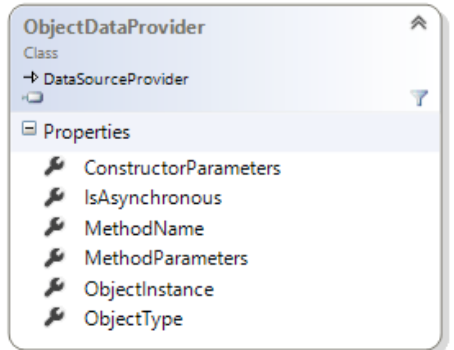
\includegraphics[scale=0.35]{ObjectDataProvider.png}
\begin{lstlisting}[language=xml]
<Window.Resources>
    <ObjectDataProvider x:Key="Alignments"
        MethodName="GetNames"
        ObjectType="{x:Type sys:Enum}">
    <ObjectDataProvider.MethodParameters>
        <x:Type TypeName="VerticalAlignment" />
    </ObjectDataProvider.MethodParameters>
    </ObjectDataProvider>
</Window.Resources>
<!-- Verwendung -->
<ComboBox ItemsSource="{Binding Source={StaticResource Alignments}}" />
\end{lstlisting}
\paragraph{DataBinding Debuggen} Man hat diverse Möglichkeiten die Abläufe hinter dem DataBinding sichtbar zu machen.
\begin{enumerate}
\item Direkt im Binding konfigurieren
\begin{lstlisting}[language=xml]
<!-- System.Diagnostics-Namespace - hinzufuegen -->
xmlns:diag="clr-namespace:System.Diagnostics;assembly=WindowsBase"
<!-- Binding Ausdruck um Setzten des TraceLevels erweitern -->
<TextBlock Text="{Binding ElementName=stack, Path=InvalidPath, diag:PresentationTraceSources.TraceLevel=High}" />
\end{lstlisting}
\item Dummy Converter schreiben
\begin{lstlisting}
public class DebugDummyConverter : IValueConverter
{
    public object Convert(object value, Type targetType, object parameter, CultureInfo culture)
    {
        return value;
    }
    public object ConvertBack(object value, Type targetType, object parameter, CultureInfo culture)
    {
        return value;
    }
}
\end{lstlisting}
\begin{lstlisting}[language=xml]
<Window.Resources> ... <local:DebugDummyConverter x:Key="MyDummy" /> ... </Window.Resources>
...
<TextBlock Text="{Binding ElementName=stack, Path=InvalidPath, Converter={StaticResource MyDummy}}" />
\end{lstlisting}
\item In VisualStudio DataBinding Debugging auf "{}All"{} setzten und im Output-Window nach \verb+Syste.Windows.Data+ suchen.
\end{enumerate}

\subsection{INotifyPropertyChanged (INPC)}
\begin{itemize}
    \item Benötigt bei: \code{OneWay}, \code{TwoWay}
    \item Nicht benötigt bei: \code{OneTime}, \code{OneWayToSource}
\end{itemize}

\subsection{RelayCommand}
''Command-Pattern'', das man selber implementieren muss, aber dann viel Zeit und Geld spart (Ziit und Geld han ich kei).

Nicht-generic RelayCommand
\begin{lstlisting}
public class RelayCommand : ICommand
{
    private readonly Action _execute;
    private readonly Func<bool> _canExecute;
    
    public RelayCommand(Action execute, Func<bool> 
        canExecute = null)
    {
        if (execute == null) throw new 
            ArgumentNullException("execute");
        
        _execute = execute;
        _canExecute = canExecute;
    }
    
    public bool CanExecute(object parameter) => 
        _canExecute?.Invoke() ?? True
    public void Execute(object parameter) => _execute();
    
    // Event an CommandManager delegieren (Benachrichtigung erfolgt
    // so immer dann wenn WPF denkt, dass sich etwas am Ausführungs- 
    // status geändert hat, z.B. bei Key- oder Mouse-Button-Klick)
    public event EventHandler CanExecuteChanged
    {
        add { CommandManager.RequerySuggested += value; }
        remove { CommandManager.RequerySuggested += value }
    }
}
\end{lstlisting}

Die Generic-Variante nutzt ein \mintinline{csharp}{Action<T>} als \mintinline{csharp}{_execute} und ein \mintinline{csharp}{Predicate<T>} als \mintinline{csharp}{_canExecute}

Verwendung:

\begin{lstlisting}
public class GadgetVm : BindableBase
{
    public ICommand SaveCommand { get; set; }
    
    public GadgetVm()
    {
        SaveCommand = new RelayCommand(
            () => this.Save(), // Methode des ViewModels
            () => this.CanSave // Property des ViewModels
        );
    }
    
    public CanSave => ; // some condition
    public void Save() {} // some method
}
\end{lstlisting}

\subsection{Multibinding}
''The new iPhone -- now only 799.00!''. Einleitendes \code{{}} wichtig!

\begin{lstlisting}
<TextBlock>
    <TextBlock.Text>
        <MultiBinding StringFormat="{}{0} -- Now only {1:0.00}!">
            <Binding Path="Description" />
            <Binding ElementName="FirstName" Path="Text" />
        </Multibinding>
    </TextBlock.Text>
</TextBlock>
\end{lstlisting}

\subsection{Binding an anderes Element (Binding Path)}
Mit diesem Code kann man den Inhalt von, z.B. einem TextBlock, an die Eingaben in, z.B. einer Textbox, binden. In diesem Beispiel machen wir dies gleich noch durch ein MultiBinding, der Binding-Ausdruck an sich ist aber allgemeingültig.

\begin{lstlisting}
<TextBox Name="FirstName" />
<TextBox Name="LastName" />
<TextBlock>
    <!-- Anzeige: "FirstName LastName" -->
    <MultiBinding StringFormat="{}{0} {1}">
        <!-- Binden an FirstName.Text -->
        <Binding ElementName="FirstName" Path="Text" />
        <Binding ElementName="LastName" Path="Text" />
    </MultiBinding>
</TextBlock>
\end{lstlisting}
\section{Benutzerinteraktion}
\paragraph{Routed Events} Events wandern vom Window den Visual Tree bis zum auslösenden Element. Routed Events besitzen meist ein Preview und ein normales Event. Das Preview Event wird ausgeführt, bevor es das Element erreicht, das normale Event, nachdem das Element das Event behandelt hat.
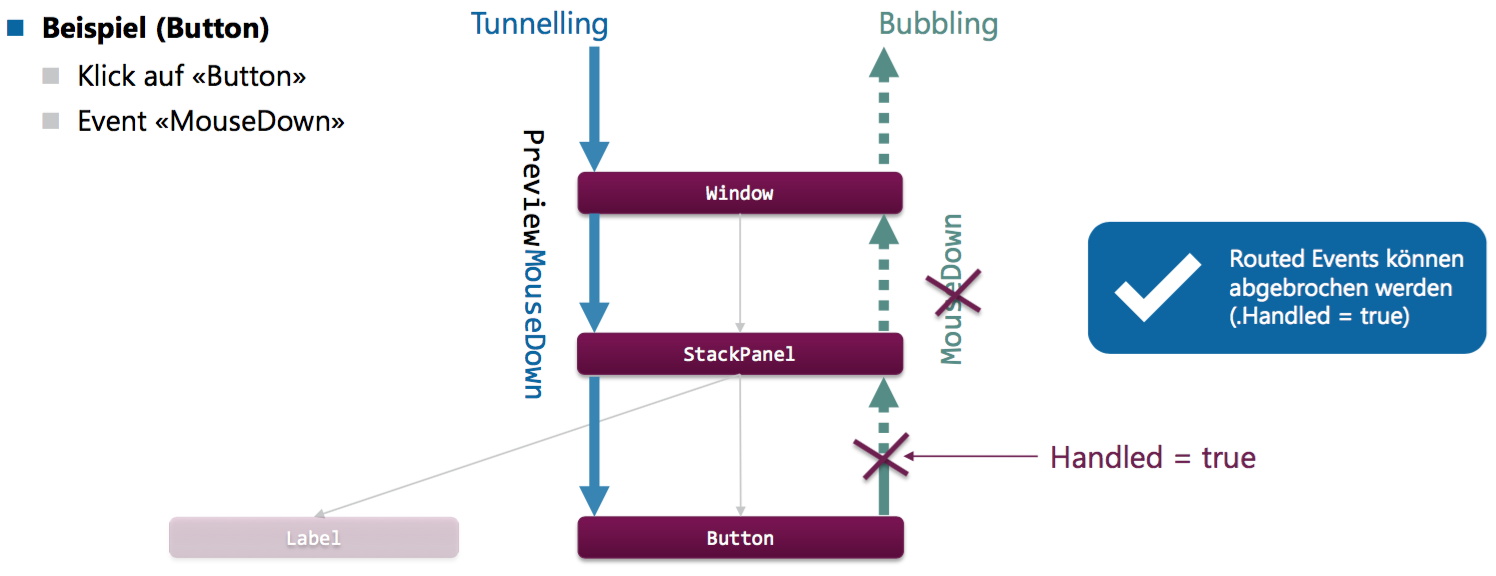
\includegraphics[scale=0.25]{RoutedEvent1.png}
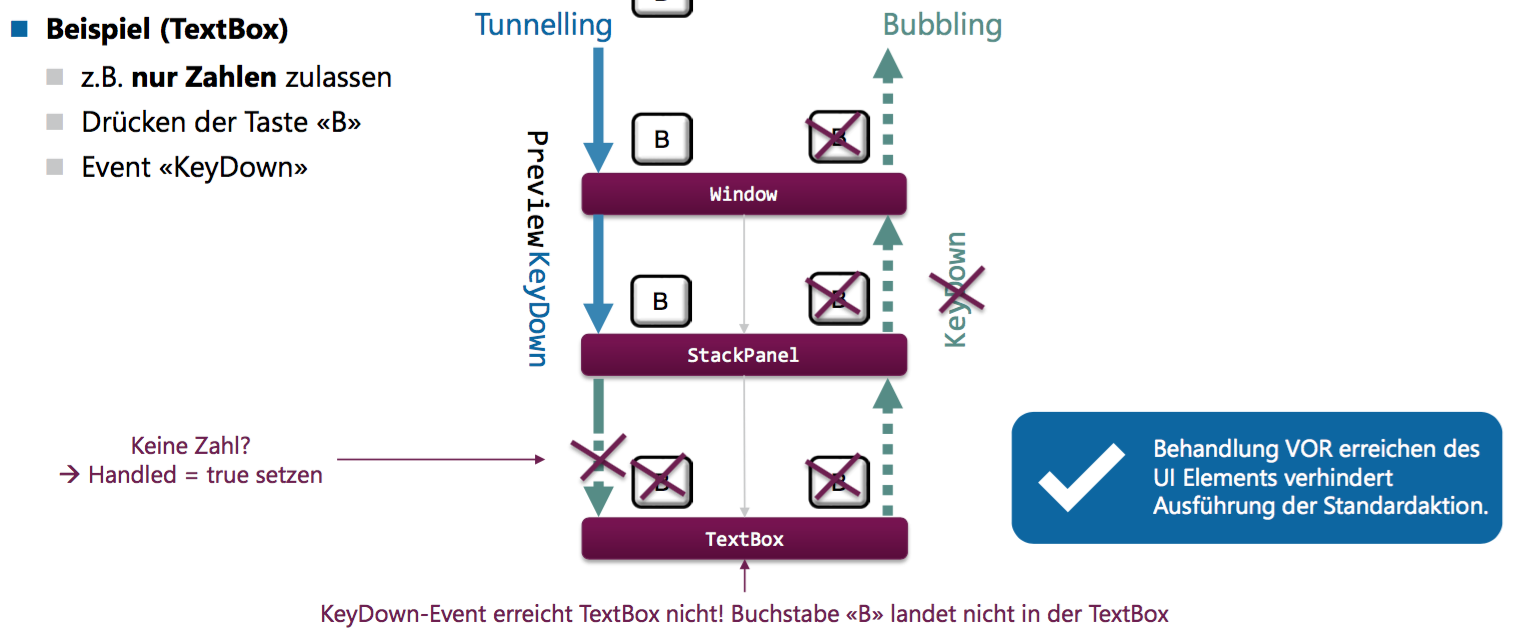
\includegraphics[scale=0.25]{RoutedEvent2.png}
Routed Events können mit \verb+Handeled = true+ unterbochen werden, sie werden dann nicht mehr weitergereicht. Man kann das Event direkt beim UI Element selbst behandeln.
\begin{lstlisting}[language=xml]
<Button Name="SaveButton"
    PreviewMouseDown="SaveButton_OnPreviewMouseDown"
    MouseDown="SaveButton_OnMouseDown">Save</Button>
\end{lstlisting}
Oder beim Parent Element
\begin{lstlisting}[language=xml]
<StackPanel PreviewMouseDown="StackPanel_OnPreviewMouseDown">
    ...
    <Button Name="SaveButton"
        PreviewMouseDown="SaveButton_OnPreviewMouseDown"
        MouseDown="SaveButton_OnMouseDown">Save</Button>
    ...
</StackPanel>
\end{lstlisting}
Eine andere Alternative wäre mit Attached Events.
\begin{lstlisting}[language=xml]
<StackPanel Button.Click="StackPanel_OnClick">
    ...
    <Button Name="SaveButton" Click="SaveButton_OnClick">Save</Button>
    ...
</StackPanel>
\end{lstlisting}
Beliebte Mouse Events:
\begin{tabular}{ll}
MouseDown & MouseEnter* \\
MouseLeave* & MouseLeftButtonDown \\
MouseLeftButtonUp & MouseMove \\
MouseRightButtonDown & MouseRightButtonUp \\
MouseUp & MouseWheel
\end{tabular}
Interessante Keyboard Events:
\begin{tabular}{ll}
KeyDown & KeyUp \\
TextInput & 
\end{tabular}
Interessante Touch-Events:
\begin{tabular}{ll}
TouchDown & TouchEnter* \\
TouchLeave* & TouchMove \\
TouchUp & 
\end{tabular}
* haben kein Preview Event.
\paragraph{RoutedEventArgs} RoutedEventArgs leiten von EventArgs ab. 
\begin{itemize}
\item \verb+Handled+: Boolean der aussagt, ob das Event behandelt wurde
\item \verb+OriginalSource+: Quell-Element (Hit-Testing) welches das Event ausgelöst hat
\item \verb+RoutedEvent+: Das RoutedEvent, welches mit diesem Objekt verknüpft ist
\item \verb+Source+: Element, welches das Event rapportiert hat
\end{itemize}
Die OriginalSource kann ein Kind-Element des Source-Elements sein, das per Hit-Testing als 1. Adressat des Events bestimmt wurde. Die Source ist das Element im Logical Tree, welches das Event rapportiert hat. Beispielsweise beim Subscribe auf MouseDown auf einem Button, wird das Event vom Button rapportiert (Source), wurde aber eigentlich vom Rahmen ausgelöst (OriginalSource).
\paragraph{Ableitende Klasse von RoutedEventArgs} Es gibt für verschiedene Input-Geräte Ableitungen von RoutedEventArgs. Auswahl von \verb+MouseEventArgs+:
\begin{itemize}
\item \textbf{LeftButton}: Zustand der linken Maustaste (Pressed/Released)
\item \textbf{MiddleButton}
\item \textbf{RightButton}
\item \textbf{Delta}: Mausradbewegung (-120/120)
\end{itemize}
Auswahl von \verb+KeyEventArgs+:
\begin{itemize}
\item \textbf{Key}: Taste (Enum)
\item \textbf{IsDown}
\item \textbf{IsUp}
\item \textbf{IsRepeat}
\item \textbf{SystemKey}: Die zusätzliche Taste, falls ALT-Taste gedrückt wurde. Key steht in \verb+Key.System+
\end{itemize}
\subsection{Drag \& Drop}
Drag \& Drop besteht aus 3 Phasen:
\begin{enumerate}
\item \textbf{Maustaste wird gedrückt:} Nach überschreiten einer Mindestdistanz wird die Aktion gestartet
\item \textbf{Während des Ziehens:} Steuerelemente unterhalb des Zeigers müssen melden, ob sie als Ziel infrage kommen
\item \textbf{Fallenlassen:} Steuerelement unterhalb des Mauszeigers muss eine Aktion mit dem bewegten Objekt durchführen
\end{enumerate}
Beispiel:
\begin{lstlisting}
public ObservableCollection<UserInfo> AvailableUsers { get; set; }
public ObservableCollection<UserInfo> SelectedUsers { get; set; }
public MainWindow()
{
    // Listen initialisieren und fuellen
    InitializeComponent();
    DataContext = this;
}
\end{lstlisting}
\paragraph{Phase 1} Maustaste wird gedrückt
\begin{lstlisting}[language=xml]
<ListBox Name="AvailableListBox" ItemsSource="{Binding AvailableUsers}"
    ItemTemplate="{StaticResource UserInfoTemplate}"
    PreviewMouseLeftButtonDown="AvailableListBox_ OnPreviewMouseLeftButtonDown"
    PreviewMouseLeftButtonUp="AvailableListBox_ OnPreviewMouseLeftButtonUp"
    MouseMove="AvailableListBox_OnMouseMove" />
\end{lstlisting}
\begin{lstlisting}
private Point? dragStartPosition = null;
private void AvailableListBox_ OnPreviewMouseLeftButtonUp(object sender, MouseButtonEventArgs e)
{
    dragStartPosition = null;
}
private void AvailableListBox_ OnPreviewMouseLeftButtonDown(object sender, MouseButtonEventArgs e)
{
    dragStartPosition = e.GetPosition(this);
}
private bool IsMovementFarEnough(Point origPos, Point curPos)
{
    var minDistX = SystemParameters.MinimumVerticalDragDistance;
    var minDistY = SystemParameters.MinimumHorizontalDragDistance;
    return (Math.Abs(curPos.X - origPos.X) >= minDistX || Math.Abs(curPos.Y - origPos.Y) >= minDistY);
}
private void AvailableListBox_OnMouseMove(object sender, MouseEventArgs e)
{
    // gar nicht starten, wenn nicht (innerhalb Liste) geklickt
    if (dragStartPosition == null)
        return;
    // aktuelle Position holen und pruefen, ob die Maus genug
    // bewegt wurde, um die Bewegung als Drag zu interpretieren
    var position = e.GetPosition(this);
    if (!IsMovementFarEnough(dragStartPosition.Value, position))
        return;
    // Alles ok, drag kann starten
    dragStartPosition = null;
    StartDrag(AvailableListBox.SelectedItem as UserInfo);
}
private void StartDrag<T>(T obj)
{
    // Bereich definieren, auf dem der Drag-Vorgang gueltig ist
    var dragScope = this.Content as FrameworkElement;
    // Container fuer Nutzdaten (hier String)
    var dragData = new DataObject(typeof(T), obj);
    // Drag-Vorgang starten
    DragDrop.DoDragDrop(dragScope, dragData, DragDropEffects.Move);
}
\end{lstlisting}
Die \verb+DragDrop.DoDragDrop+ Methode blockiert die weitere Code-Ausführun bis die Operation beendet ist.
\paragraph{Phase 2} Maus wird gezogen
\begin{lstlisting}[language=xml]
<ListBox Name="SelectedListBox" ItemsSource="{Binding SelectedUsers}"
    ItemTemplate="{StaticResource UserInfoTemplate}"
    AllowDrop="True"
    DragOver="SelectedListBox_OnDragOver"
    Drop="SelectedListBox_OnDrop" />
\end{lstlisting}
\begin{lstlisting}
private void SelectedListBox_OnDragOver(object sender, DragEventArgs e)
{
    // Objekt auspacken
    var data = e.Data.GetData(typeof(UserInfo)) as UserInfo;
    // falls Objekt verfuegbar, dann kopieren, sonst keine Operation
    e.Effects = data != null ? DragDropEffects.Copy : DragDropEffects.None;
}
\end{lstlisting}
\paragraph{Phase 3} Objekt wird fallengelassen
\begin{lstlisting}[language=xml]
<ListBox Name="SelectedListBox" ItemsSource="{Binding SelectedUsers}"
    ItemTemplate="{StaticResource UserInfoTemplate}"
    AllowDrop="True"
    DragOver="SelectedListBox_OnDragOver"
    Drop="SelectedListBox_OnDrop" />
\end{lstlisting}
\begin{lstlisting}
private void SelectedListBox_OnDrop(object sender, DragEventArgs e)
{
    // Objekt auspacken
    var user = e.Data.GetData(typeof(UserInfo)) as UserInfo;
    // Dank Data Binding reicht es nun, das UserInfo Objekt
    // der ObservableCollection hinzuzufuegen:
    SelectedUsers.Add(user);
}
\end{lstlisting}
\paragraph{Drag \& Drop Events}
\begin{itemize}
\item \textbf{DragEnter:} Tritt auf, wenn dieses Element während einer Drag-Operation als Drag Target fungieren würde (Hit-Testing)
\item \textbf{DragLeave:} Tritt auf, wenn dieses Element während einer Drag-Operation verlassen wird
\item \textbf{DragOver:} Tritt auf, wenn diesem Element eine Drag-Operation stattfindet
\item \textbf{Drop:} Tritt auf, wenn das Objekt der Drag-Operation auf dieses Element fallengelassen wird
\item \textbf{GiveFeedback:} Gibt der Quelle der Drag-Operation eine Chance, visuelles Feedback zu geben
\end{itemize}
\section{Hintergrund-Operationen}
Lange Dauernde Operationen sollten nicht im UI-Thread ausgeführt werden, sonden in ein eigenen Thread ausgelagert werden, sodass das UI nicht einfriert. Um den Benutzer zu informieren, dass irgendwas "{}arbeitet"{} sollte man folgendermassen vorgehen:
\begin{enumerate}
\item Visuelles Feedback geben (Spinner, Overlay, Popup), wenn nötig
\item Starten eines Background-Threads als Reaktion auf ein Event, Kontrolle an UI Thread zurückgeben
\item Bei Thread-Ende aus dem Background-Thread den UI-Thread benachrichtigen
\end{enumerate}
\paragraph{Visuelles Feedback} Das visuelle Feedback umfasst auch, dass der Benutzer dieselbe Operation nicht aus versehen zweimal ausführt. Dies verhindert man, indem man beispielsweise den Button deaktiviert etc. Um dem Benutzer mittzuteilen, dass etwas läuft, kann man beispielsweise ein Spinner auf den Button legen (realisierbar durch Grid innerhalb des Buttons). 
%TODO: Eventuell noch XAML Beispiel
\paragraph{Starten eines Background Threads} Dazu verwendet man am besten die Task Paralell Library. 
\begin{lstlisting}
Task.Run(() => {
    //Background operation
});
\end{lstlisting}
\paragraph{UI-Thread benachrichtigen} Mit der TPL kann man einen Dispatcher verwenden, um Code im UI-Thread auszuführen.
\begin{lstlisting}
Task.Run(() => {
    //Background operation
    Dispatcher.Invoke(() => {
        // UI interaktion
    });
});
\end{lstlisting}
Falls Dispatcher nicht aus Code-Behind aufgerufen wird (Dispatcher ist eine Property der UI-Elemente wie Window, muss man stattdessen \verb+System.Windows.Threading.+
\verb+Dispatcher.CurrentDispatcher+ verwenden.
\section{CUIT}
Annahmen: es gibt ein Fenster mit \code{Title="Login Window"}. In diesem Fenster gibt es zwei \code{Textbox}en mit LoginName und Password (Attribut \code{Name=}), und einen \code{Button} der sich LoginButton nennt. Stimmt das Login, so öffnet sich ein Fenster mit dem Titel \code{"Welcome Window"}, welches ein \code{Label} mit dem Namen NameLabel besitzt.

Wir wollen nun den Usernamen und das Passwort abfüllen, OK klicken, und sehen ob das korrekte Fenster aufgeht.

\begin{lstlisting}
[TestClass]
public class LoginWindowUiTest
{
  // Das Folgende kann immer gleich implementiert werden
  // the directory in which the test is running
  public string BaseDir => Path.GetDirectoryName(Assembly.GetExecutingAssembly().Location);
  // system under test (wpf app to be tested)
  public string SutPath => Path.Combine(BaseDir, $"ch.hsr.wpf.03.login.exe");
  
  [TestMethod]
  public void TestMethod1()
  {
  var app = Application.Launch(SutPath);
  var window = app.GetWindow("Login Window", InitializeOption.NoCache);
  var name = window.Get<TextBox>("LoginName");
  var pw = window.Get<TextBox>("Password");
  name.Text = "j.bond";
  pw.Text = "topsecret";
  var button = window.Get<Button>("LoginButton");
  button.Click();
  var win = app.GetWindow("Welcome Window", InitializeOption.NoCache);
  var label = win.Get<Label>("NameLabel");
  Assert.AreEqual("j.bond", label.Text);
  win.Close();
  app.Close();
  }
  
}
\end{lstlisting}

\subsection{INotifyPropertyChanged}

\begin{lstlisting}[language=java]
// Clock.cs
public class Clock:INotifyPropertyChanged
{
  private DateTime _time;
  public DateTime Time {
    get { return _time; }
    set
    {
      if (value != _time)
      {
        _time = value;
    
        OnPropertyChanged(nameof(Time));
        OnPropertyChanged(nameof(TimeString));
      } 
    }
  }
  public string TimeString => Time.ToString("dd.MM.yyyy HH:mm:ss");
  public Clock()
  {
    Time = DateTime.Now;
  }
  public event PropertyChangedEventHandler PropertyChanged;
  protected virtual void OnPropertyChanged(string propertyName = null)
  {
    PropertyChanged?.Invoke(this, new PropertyChangedEventArgs(propertyName));
  }
}

//App.xaml.cs
public partial class App : Application
{
  public DispatcherTimer Timer { get; set; }
  public Clock Clock { get; set; }
  protected override void OnStartup(StartupEventArgs e)
  {
    Clock = new Clock();
    Timer = new DispatcherTimer();
    // Jede Sekunde das Tick-Event auslösen:
    Timer.Interval = TimeSpan.FromSeconds(1);
    Timer.Tick += (sender, args) =>
    {
      // Do something...
      Clock.Time = DateTime.Now;
    };
    Timer.Start();
    MainWindow = new MainWindow();
    MainWindow.DataContext = Clock;
    MainWindow.Show();
  }
}
\end{lstlisting}

\begin{lstlisting}[language=xml]
<!-- MainWindow.xaml -->
<Label ... Content="{Binding TimeString}" />
\end{lstlisting}

\section{MVVM}
\paragraph{Model} Eigentliche Daten, Domain Objekte Kein
Verhalten, Nicht zuständig für Formatierung, Nicht zu zuständig für Laden und Speichern
\paragraph{ViewModel} View-Spezifische Objekte, welche Model um Daten/Berechnete Fields erweitern Enthalten Verhalten. Grundlage für DataBinding. Kontroverse bezgl. Laden. Kennt View nicht
\paragraph{View} XAML + Code Behind(Wenig). Nutzt Binding z.B. Button->Commands, TextBox->String, Event->Command(Benötigt Library)
\paragraph{Anmerkung} Auf Interfaces Referenzieren die eine andere Komponente implementiert ist ok.
\paragraph{StartupCode} Wer erstellt VMs, Vs und lädt Ms? Spezielles AppVM verwenden, welches beim Start erzeugt wird. Zusätzliche VMs werden vom APPVM erzeugt (Factory). Views werden direkt innerhalb der View erzeugt. VM erzeugt, lädt und speichert Ms

\begin{lstlisting}
// App.xaml Startup Uri entfernen

// App Class
public AppVm {get; set; }
protected override void onStartup(StartupEventArgs e)
{
    base.OnStartup(e);
    AppVm = new AppVm
    
    // hier: eine der Varianten unten
}

MainWindow = new MainView();
MainWindow.Show();

var vm = new ViewModel();
MainWindow = MainView();
MainView.DataContext = vm;
MainWindow.Show();
\end{lstlisting}
\end{multicols*}
\end{document}
